\documentclass[12pt,a4paper]{article}
\usepackage[utf8x]{inputenc}
\usepackage{ucs}
\usepackage[MeX]{polski}
\usepackage{fancyhdr}
\usepackage{amsmath}
\usepackage{amsfonts}
\usepackage{amssymb}
\pagestyle{plain}
\usepackage{enumerate}
\usepackage{listings}
\usepackage{graphicx}
%\usepackage{subfig}
\usepackage{caption}
\usepackage{float}
\usepackage{tabularx}
\usepackage{nameref}
\usepackage{subcaption}

% Poniższy fragment preambuły by Piotr Matuszak.
\usepackage[polish]{babel} %język polski
%\usepackage[utf8]{inputenc} %interpretacja znaków
\usepackage[T1]{fontenc} %interpretacja polskich znaków
\usepackage{lmodern} 
\usepackage[margin=2cm]{geometry} %marginesy
%\usepackage[]{natbib} %bibliografia
\usepackage{graphicx} %wstawianie obrazów i do tablicy
%usepackage{wrapfig} %obrazy przyległe do tekstu
%\usepackage{mathtools}  %funkcje matematyczne
%\mathtoolsset{showonlyrefs} %nienumerowanie wzorów matematycznych
\usepackage{float}
\usepackage{booktabs} % do tablicy
\usepackage{multirow} % do tablicy
\usepackage{enumitem}  % tryb listy [pogrubiony tekst] [wyjasnienie] 
\usepackage[font=small]{caption} % podpisy małe
\usepackage[font=small]{subcaption} % subpodpisy małe
\usepackage[pdftex,hidelinks]{hyperref} % href, ukrywa czerwone obwódki wokół linków
\usepackage[table,xcdraw]{xcolor}
\usepackage{lscape}
\pagestyle{plain} % zwykły tekst
%\usepackage{indentfirst} %pierwszy paragraf z wcięciem
\usepackage{tabularx} %tablica o zadanej szerokości
%\usepackage{makecell}
\usepackage{listings}
%\usepackage{mdframed}

\lstset{
	basicstyle=\footnotesize,        % the size of the fonts that are used for the code
	breakatwhitespace=false,         % sets if automatic breaks should only happen at whitespace
  	breaklines=true,                 % sets automatic line breaking
  	frame=single,	                 % adds a frame around the code
  	numbers=left,                    % where to put the line-numbers; possible values are (none, left, right)
  	numbersep=5pt,                   % how far the line-numbers are from the code
  	numberstyle=\tiny,					 % the style that is used for the line-numbers
  	tabsize=2,	                   % sets default tabsize to 2 spaces
}

\definecolor{codegreen}{rgb}{0,0.6,0}
\definecolor{codegray}{rgb}{0.5,0.5,0.5}
\definecolor{codepurple}{rgb}{0.58,0,0.82}
\definecolor{backcolour}{rgb}{0.95,0.95,0.92}
\definecolor{framecolour}{rgb}{0.58, 0.741, 0.835}

\lstloadlanguages{Fortran,C++,C,[LaTeX]TeX,Python,bash,R, Perl}

\renewcommand{\lstlistingname}{Polecenie}% Listing -> Algorithm
\renewcommand{\lstlistlistingname}{Lista poleceń}% List of Listings -> List of Algorithms

  \lstset{%
    language=bash,
    otherkeywords={=, +, [, ], (, ), \{, \}, *},
    % bash commands from:
    %http://www.math.montana.edu/Rweb/Rhelp/00Index.html
    emph={addgroup,adduser,alias,
    ant,
    apropos,apt-get,aptitude,aspell,awk,
    basename,bash,bc,bg,break,builtin,bzip2,cal,case,cat,cd,cfdisk,chgrp,
    chkconfig,chmod,chown,chroot,cksum,clear,cmp,comm,command,continue,
    cp,cron,crontab,csplit,cut,date,dc,dd,ddrescue,declare,df,diff,diff3,
    dig,dir,dircolors,dirname,dirs,dmesg,du,echo,egrep,eject,enable,env,
    ethtool,eval,exec,exit,expand,expect,export,expr,false,fdformat,
    fdisk,fg,fgrep,file,find,fmt,fold,for,format,free,fsck,ftp,function,
    fuser,gawk,getopts,
    git,
    grep,groups,gzip,
    gunzip,
    ,hash,head,help,history,hostname,
    id,if,ifconfig,ifdown,ifup,import,install,
    java, java6, java_cur
    join,kill,killall,less,
    let,ln,local,locate,logname,logout,look,lpc,lpr,lprint,lprintd,
    lprintq,lprm,ls,lsof,make,man,mkdir,mkfifo,mkisofs,mknod,mmv,more,
    mount,mtools,mtr,mv,
    mysql,
    netstat,nice,nl,nohup,notify-send,
    noweb,noweave,
    nslookup,op,
    open,passwd,paste,pathchk,ping,pkill,popd,pr,printcap,printenv,
    printf,ps,pushd,pwd,quota,quotacheck,quotactl,ram,rcp,read,
    readarray,readonly,reboot,remsync,rename,renice,return,rev,rm,rmdir,
    rsync,scp,screen,sdiff,sed,select,seq,set,sftp,shift,shopt,shutdown,
    sleep,slocate,sort,source,split,ssh,strace,su,sudo,sum,
    svn, svn2git,
    symlink,sync,
    tail,tar,tee,test,time,times,top,touch,tr,traceroute,trap,true,
    tsort,tty,type,ulimit,umask,umount,unalias,uname,unexpand,uniq,
    units,
    unrar,
    unset,unshar,until,useradd,usermod,users,uudecode,uuencode,
    vdir,vi,vmstat,watch,wc,Wget,whereis,which,while,who,whoami,write,
    zcat},
    breaklines=true,
    keywordstyle=\color{blue},
    stringstyle=\color{red},
    emphstyle=\color{black}\bfseries,
    commentstyle=\color{gray}\slshape,
  }

\lstdefinestyle{mystyle}{
    backgroundcolor=\color{backcolour},   
    commentstyle=\color{codegreen},
    keywordstyle=\color{magenta},
    numberstyle=\tiny\color{codegray},
    stringstyle=\color{codepurple},
    basicstyle=\footnotesize,
    breakatwhitespace=false,         
    breaklines=true,                 
    captionpos=b,                    
    keepspaces=true,                 
    %numbers=left,                    
    numbers=none,
    numbersep=5pt,                  
    showspaces=false,                
    showstringspaces=false,
    showtabs=false,                  
    tabsize=2
}

%Dokumentacja techniczna projektu Rękawica Sensoryczna 2017
\usepackage{graphicx}
\usepackage{hyperref}


\renewcommand{\maketitle}{\begin{titlepage}

\begin{center}


\LARGE\centering Dokumentacja techniczna projektu Rękawica Sensoryczna\\
\large\centering Projekt realizowany w ramach kursu Roboty Mobilne 1 na Politechnice Wrocławskiej\\
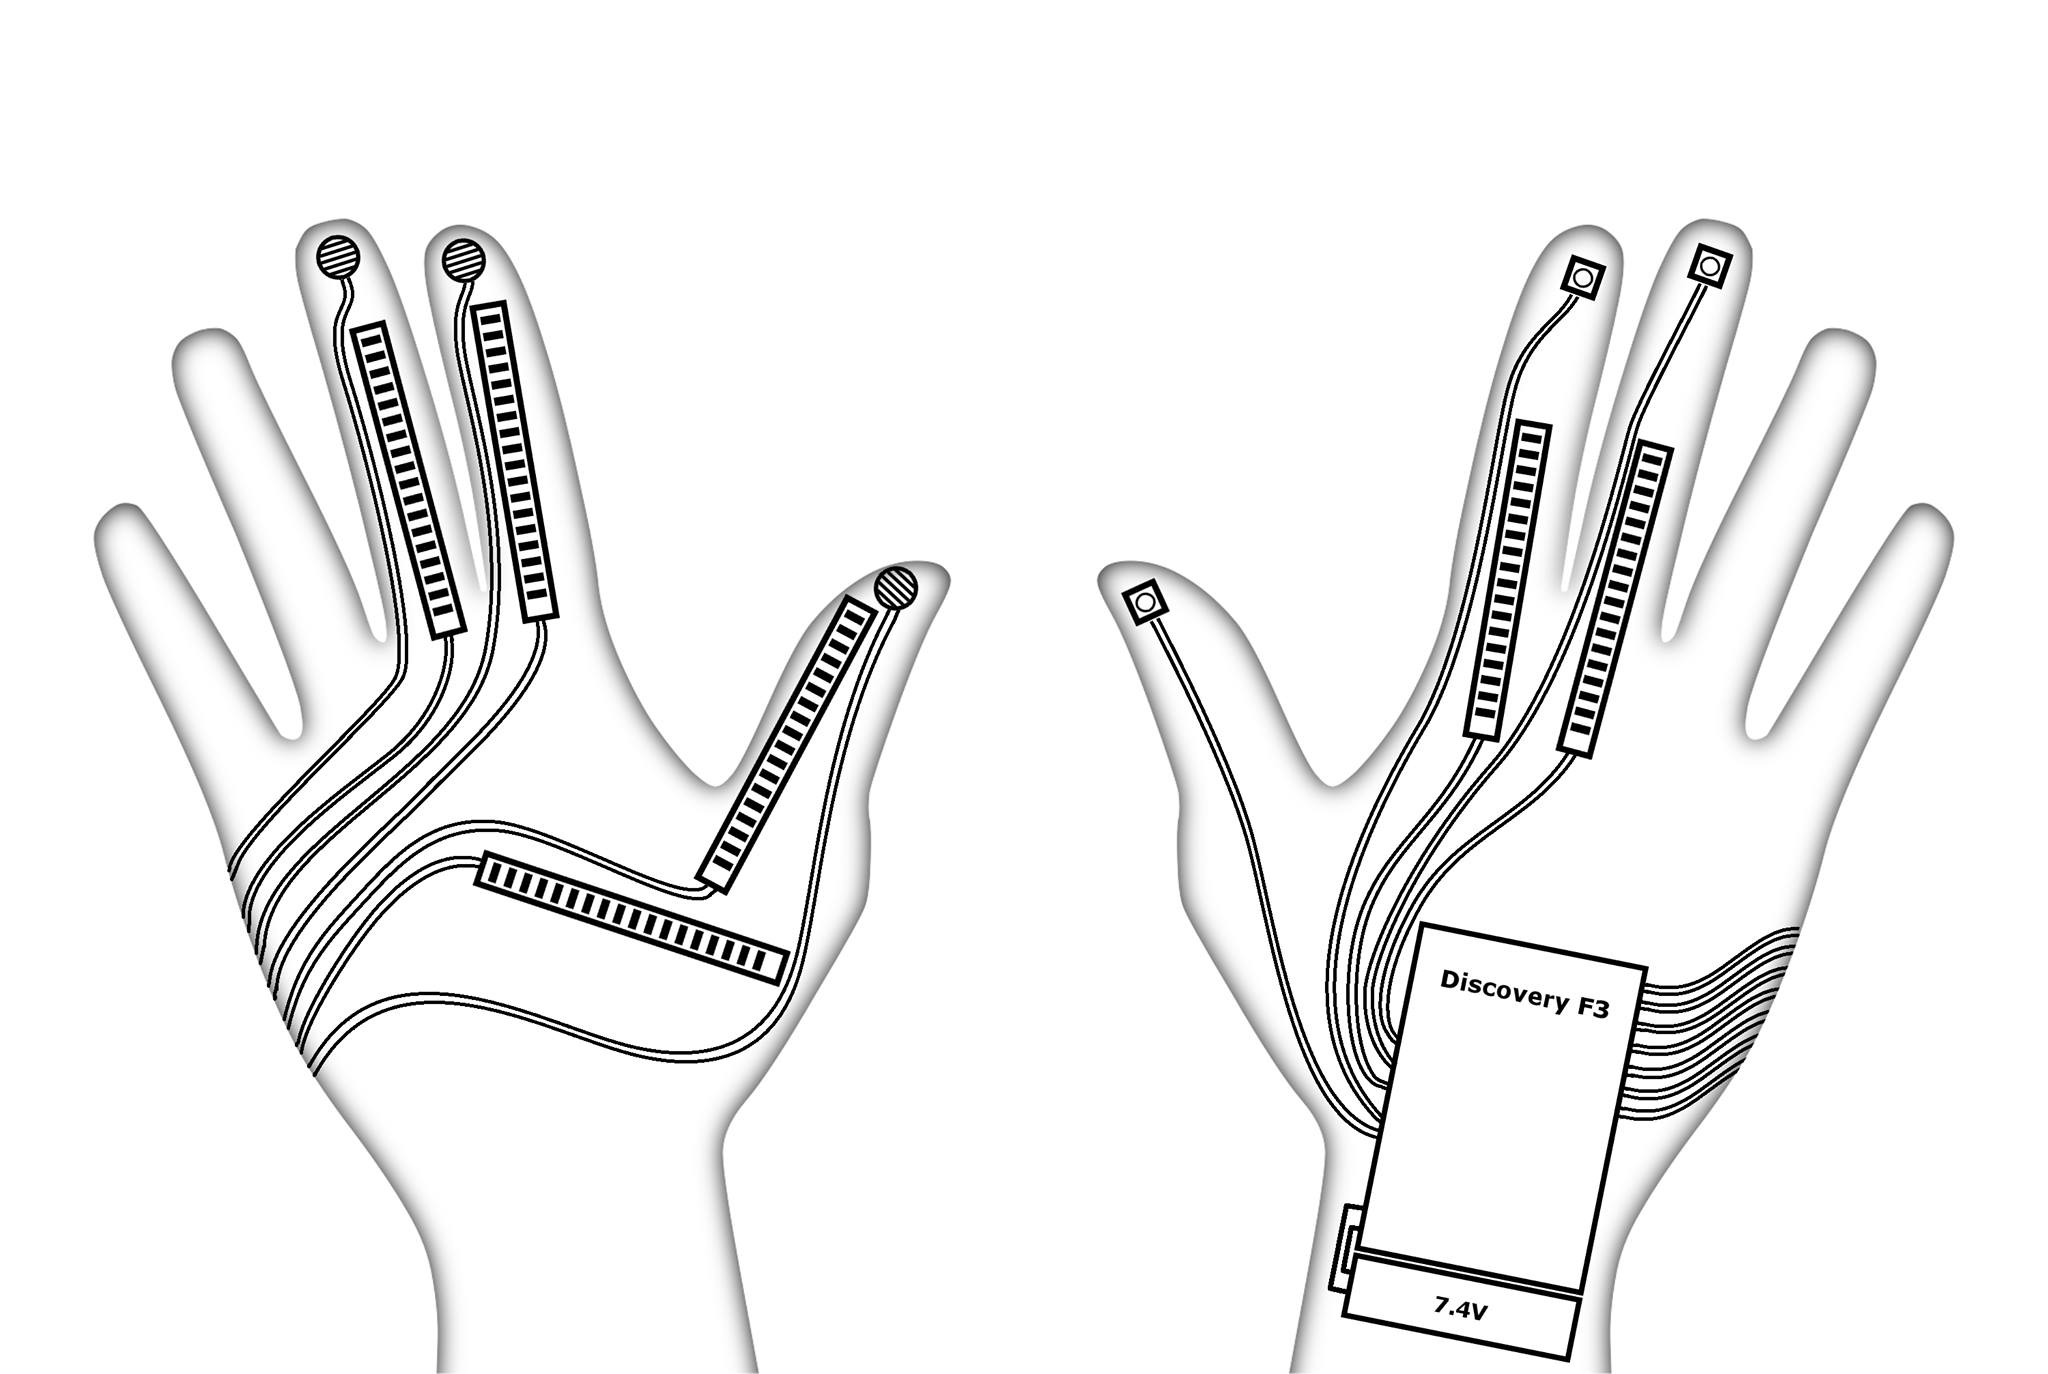
\includegraphics[width=0.7\textwidth]{images/rekawica_old.jpg}
\vspace*{2cm}
\normalsize\flushleft\textbf{Temat Projektu:} Rękawica sensoryczna\\
\textbf{Autorzy:} Krzysztof Dąbek 218549, Dymitr Choroszczak 218627,\\Anna Postawka 218556\\
\textbf{Kierunek:} Automatyka i Robotyka\\
\textbf{Specjalność:} Robotyka (ARR)\\
\textbf{Prowadzący:} dr inż. Andrzej Wołczowski\\
\textbf{Kurs:} Roboty Mobilne 1\\
\textbf{Termin zajęć:} pn TN 11:15, śr TN 14:30\\
\vspace{5 mm}



\vspace*{3.5cm}
\centering\textsc{\today}\\

\end{center}
\end{titlepage}
\newpage
}
\begin{document}
\maketitle
\tableofcontents
\newpage


\section{Główne założenia projektowe: }\normalsize
\begin{itemize}
\item Stworzenie rękawicy z czujnikami ugięcia w trzech palcach oraz czujnikami nacisku na opuszkach
\item Zamontowanie na opuszkach LEDów (np. RGB) wizualizujących odczyty z czujników nacisku
\item Wykorzystanie płytki STM32F3Discovery do przetwarzania danych
\item Użycie akcelerometru zawartego na płytce do określenia położenia dłoni względem pionu (wektora przyśpieszenia grawitacyjnego)
\item Bezprzewodowe przesyłanie danych do komputera za pomocą modułu Bluetooth HC-06
\item Przewodowe przesyłanie danych do komputera za pomocą interfejsu USB
\item Zewnętrzne zasilanie z akumulatora
\item Uproszczony model dłoni w wizualizacji 3D
\end{itemize}

\section{Opis czujników}
\begin{itemize}
\item Na opuszkach palców zamontowano \textbf{czujniki nacisku FSR-400 Short od Interlink Electronics}. Spadek rezystancji przy przyłożonej sile pozwala zmierzyć siłę nacisku [rys. \ref{fig:wykresy_fsr-400}].
\item Do wykrycia zgięcia stawów międzypaliczkowych i śródręczno-paliczkowych oraz stawów kciuka zastosowano \textbf{czujniki ugięcia -- Flex Sensory 2.2" firmy Spectra Symbol}. Zgięcie tych sensorów powoduje wzrost rezystancji.
\item \textbf{Akcelerometr LSM303DLHC}, znajdujący się na płytce Discovery został użyty do określenia orientacji rękawicy względem wektora grawitacji.
\end{itemize}
\subsection{Parametry}
Patrz: Tabela \ref{table:tabela_fsr-400}, Tabela \ref{table:tabela_flexsensor}, Tabela \ref{table:tabela_akcelerometr}.
\subsubsection{Dane czujnika nacisku}
\begin{itemize}
\item Średnica powierzchni czynnej: 5 mm
\item Zakres pomiarowy nacisku: 0.2 - 20 N
\item Zakres rezystancji: 150 Ohm - 10 MOhm
\item Rezystor pomiarowy do dzielnika: 3 kOhm
\end{itemize}
\subsubsection{Dane czujnika ugięcia}
\begin{itemize}
\item Długość powierzchni czynnej: 55.37 mm
\item Zakres rezystancji: 25 kOhm - 125 kOhm
\item Rezystor pomiarowy do dzielnika: 62 kOhm
\end{itemize}
\subsubsection{Dane z akcelerometru}
\begin{itemize}
\item Protokół komunikacyjny: $I^2C$
\item Ilość osi: 3
\item Maksymalne przeciążenie: 16g
\item Dokładność pomiaru: 16 bitów 
\end{itemize}
\subsection{Odczyt danych z czujników}
\subsubsection{Czujniki nacisku} \label{czujniki_nacisku}
Dane z czujników są odczytywane za pomocą przetwornika ADC oraz przy użyciu DMA (Direct Memory Access), co pozwala na bezpośrednie przekierowanie danych z czujników do odpowiednich zmiennych, bez wywoływania dodatkowej funkcji zwracającej wynik pomiaru.
\subsubsection{Czujniki ugięcia}
Obsługa taka sama jak w: \nameref{czujniki_nacisku}.
\subsubsection{Akcelerometr}
Z akcelerometrem komunikacja następuje po interfejsie I$^2$C.

\begin{figure}[!htb]
\centering
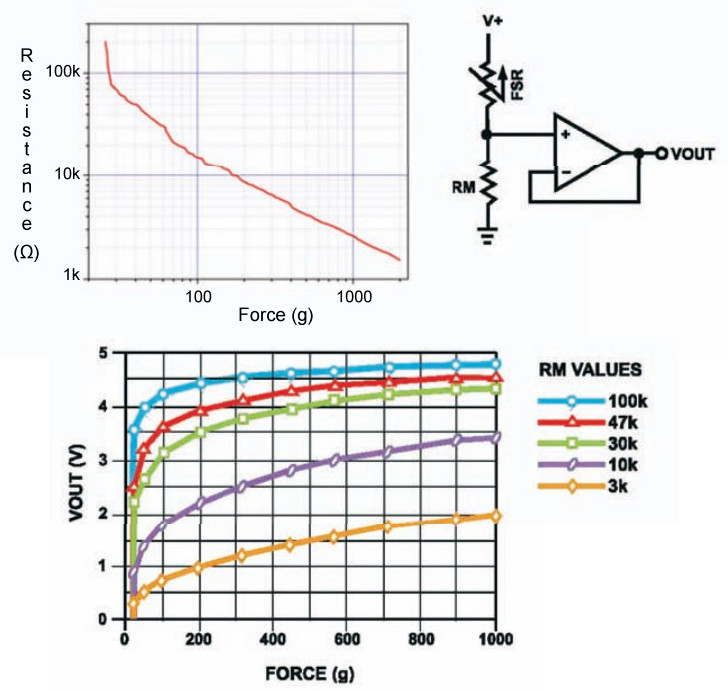
\includegraphics[width=0.8\textwidth]{images/fsr-400.jpg}
\caption{Układ pomiarowy oraz wykresy zależności napięć i rezystancji od przyłożonej siły dla czujnika FSR-400}
\label{fig:wykresy_fsr-400}
\end{figure}

\begin{table}[!htb]
\centering
\begin{tabularx}
{\textwidth}{ |X|X| }
\hline
Zakres & 0,2--20 N \\
\hline
Masa & 0,15 g \\ 
\hline
Wymiary zewnętrzne & 7,6 x 7,6 x 0,4 mm \\
\hline
\end{tabularx}
\caption{Czujnik siły nacisku FSR-400}
\label{table:tabela_fsr-400}
\end{table}


\begin{table}[!htb]
\centering
\begin{tabularx}
{\textwidth}{ |X|X| }
\hline
Min. wartość rezystancji & 25 k$\Omega$ \\
\hline
Zakres rezystancji podczas zginania & 45--125 k$\Omega$ \\
\hline
Dł. całkowita & 73,66 mm \\
\hline
Dł. użyteczna czujnika & 55,37 mm \\ 
\hline
Szerokość & 6,35 mm \\
\hline
\end{tabularx}
\caption{Czujnik ugięcia Flex Sensor 2.2"}
\label{table:tabela_flexsensor}
\end{table}


\begin{table}[!htb]
\centering
\begin{tabularx}
{\textwidth}{ |X|X| }
\hline
Napięcie pracy & 2,2--3,6 V \\
\hline
Interfejs komunikacyjny & I$^2$C \\
\hline
Rozdzielczość & 16 bitów \\
\hline
Regulowany zakres akcelerometru &  $\pm$2g, $\pm$4g, $\pm$8g, $\pm$16g \\ 
\hline
Zakres magnetometru &  od $\pm$1,3 do $\pm$8,1 gauss \\ 
\hline
\end{tabularx}
\caption{LSM303DLHC -- 3-osiowy akcelerometr i magnetometr I2C}
\label{table:tabela_akcelerometr}
\end{table}

\section{Elementy składowe projektu}

\subsection{Hardware}
Rękawica sensoryczna zbiera dane z prawej dłoni. Czujniki ugięcia przyszyto na zewnętrznej stronie dłoni [rys. \ref{fig:gotowa}].
 Przetestowano kilka ustawień czujników i takie zdaje się najlepiej spełniać założenia, czyli poprawnie odczytywać zgięcia konkretnych stawów palców, nie ograniczając przy tym ruchów dłoni. Czujniki nacisku przymocowano na opuszkach [rys. \ref{fig:gotowa2}]. Zostały one przyklejone klejem błyskawicznym. Przymocowano również na wierzchu dłoni 2 listwy żeńskie do wpięcia płytki Discovery F3, aby móc pobierać dane z akcelerometru i wykrywać obrót ręki [rys. \ref{fig:gotowa}].
 
\begin{figure}[!htb]
\centering
\begin{subfigure}{.5\textwidth}
	\centering
	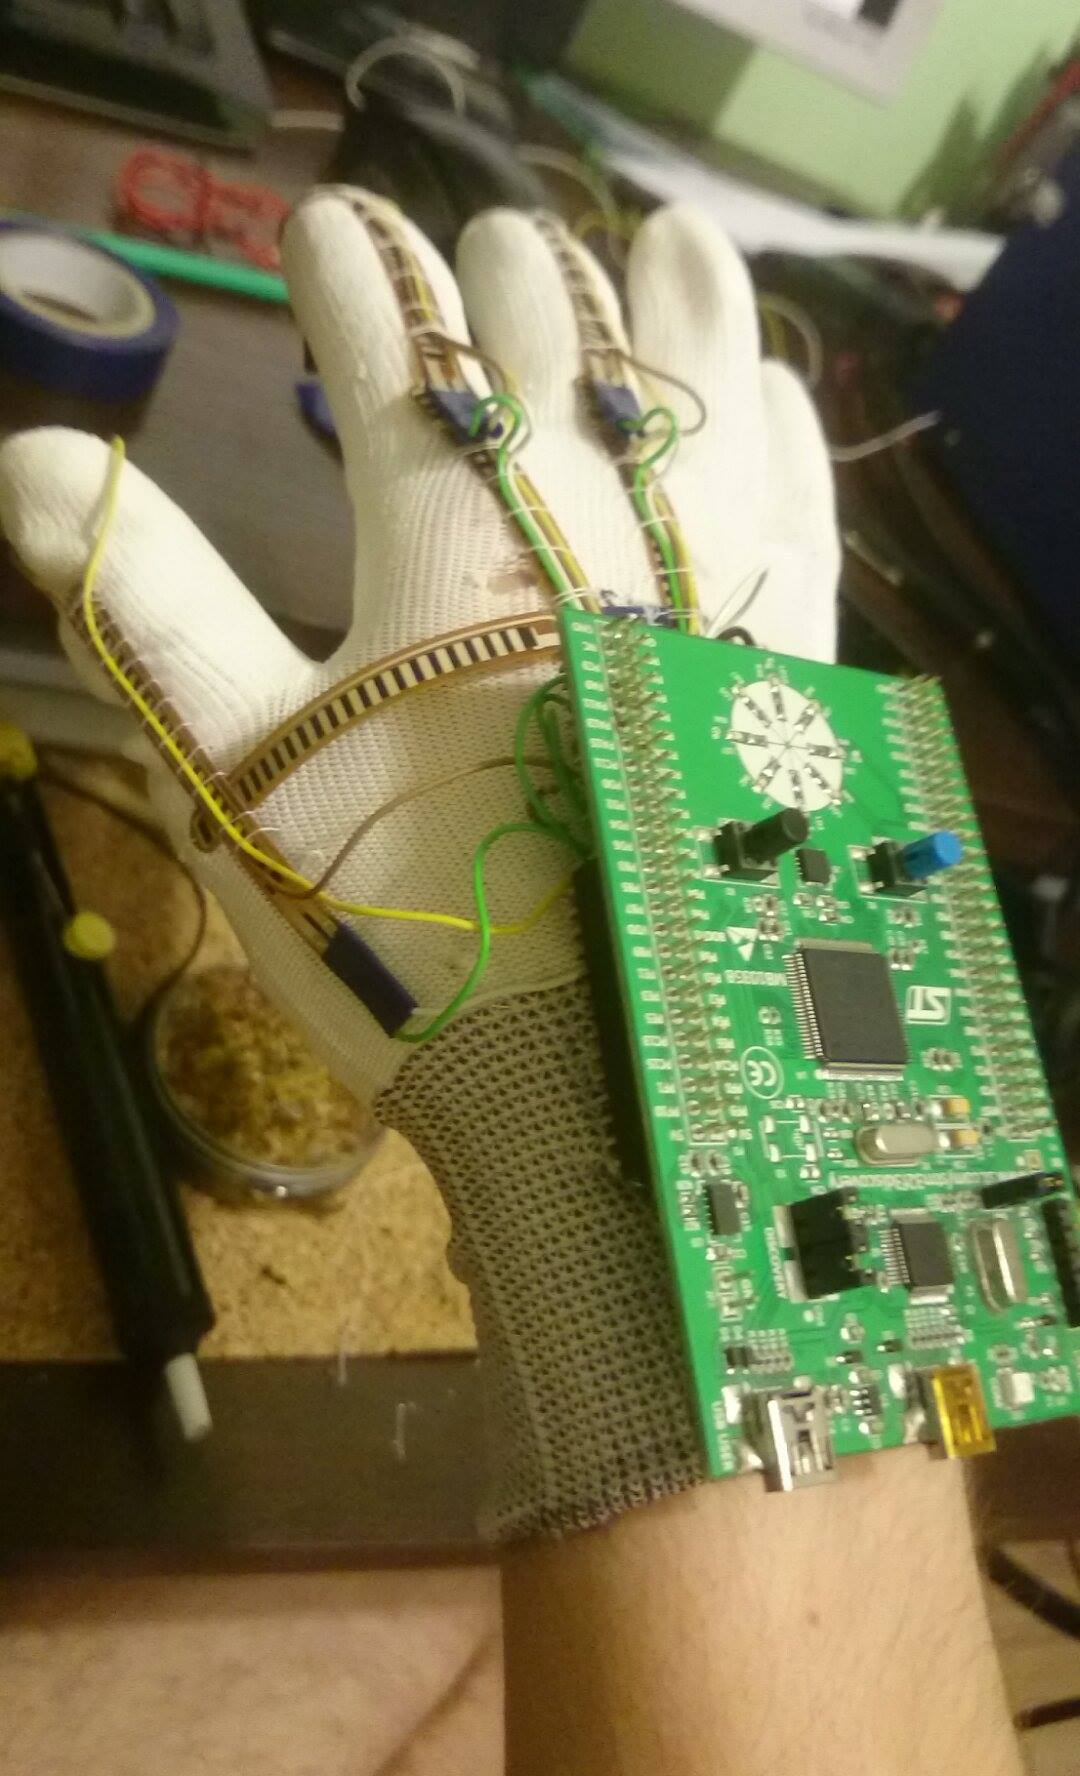
\includegraphics[width=.9\textwidth]{images/gotowa.jpg}
	\caption{Zewnętrzna część dłoni}
	\label{fig:gotowa}
\end{subfigure}%
\begin{subfigure}{.5\textwidth}
	\centering
	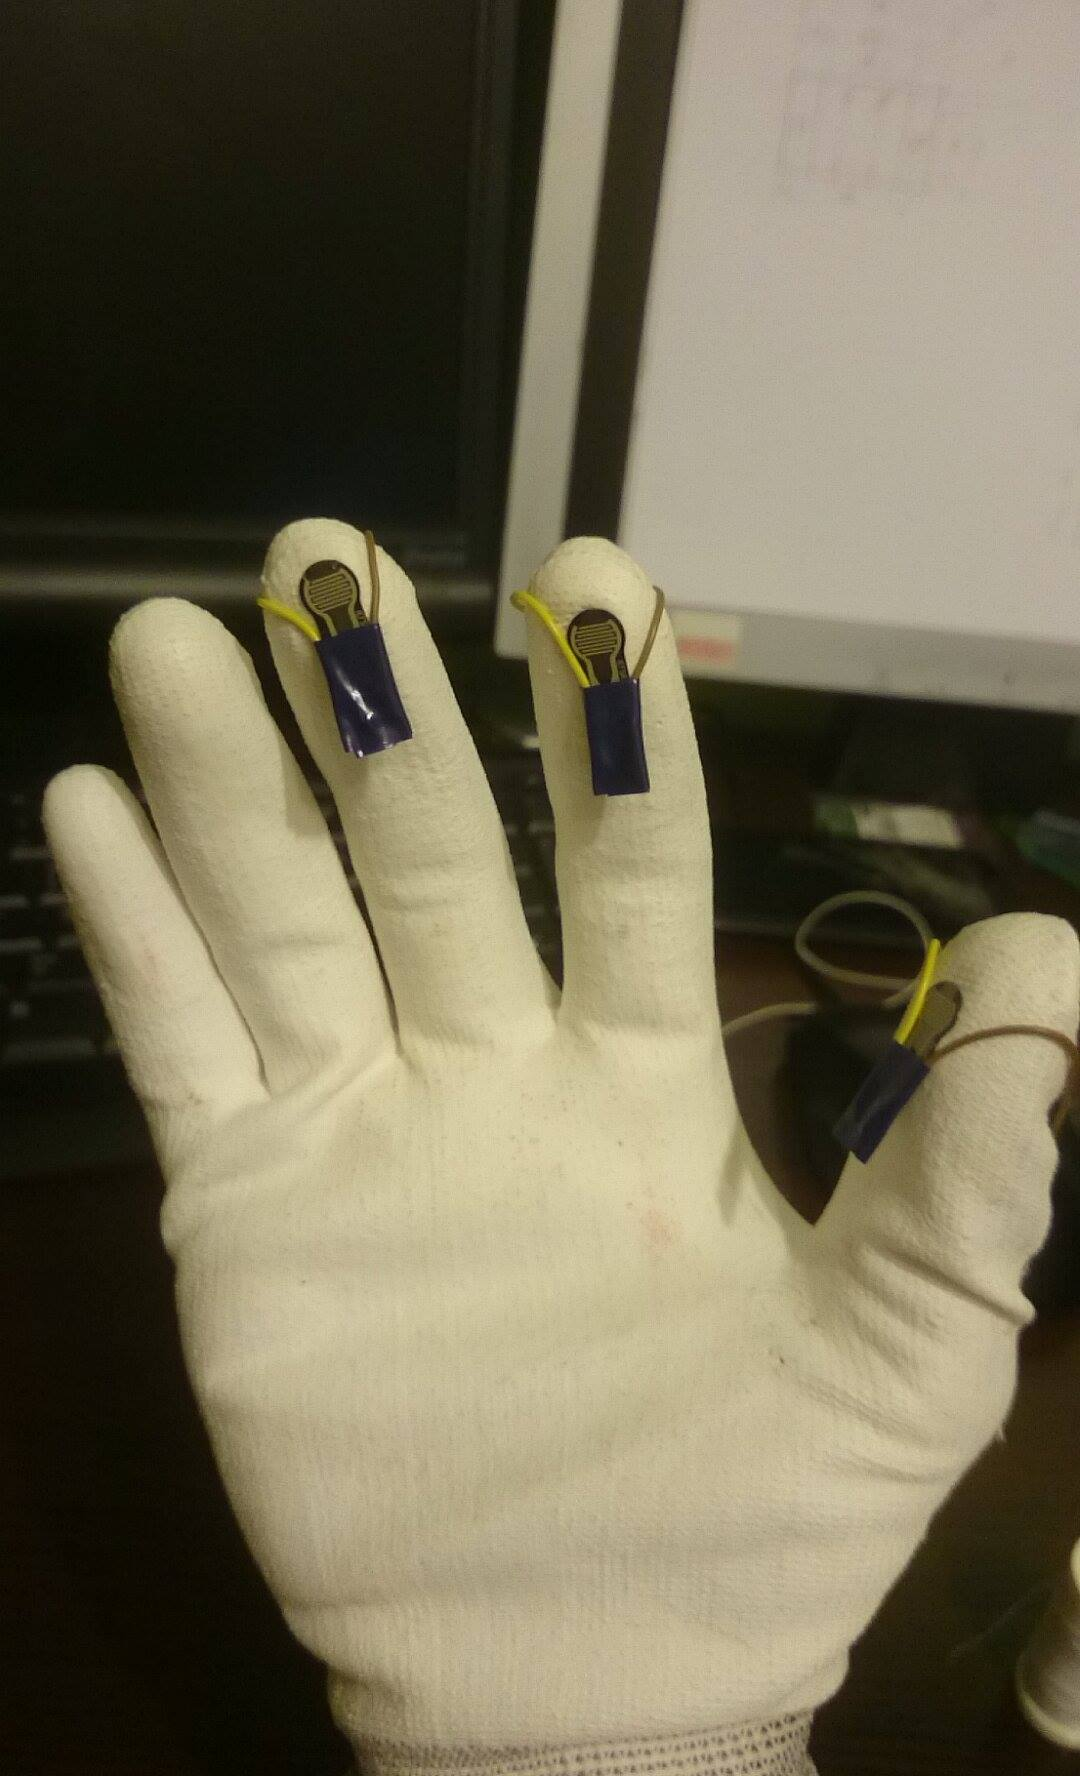
\includegraphics[width=.9\textwidth]{images/gotowa2.jpg}
	\caption{Wewnętrzna część dłoni}
	\label{fig:gotowa2}
\end{subfigure}
\caption{Gotowa rękawica}
\label{fig:gotowa_rekawica}
\end{figure}


\begin{figure}[h]
\centering
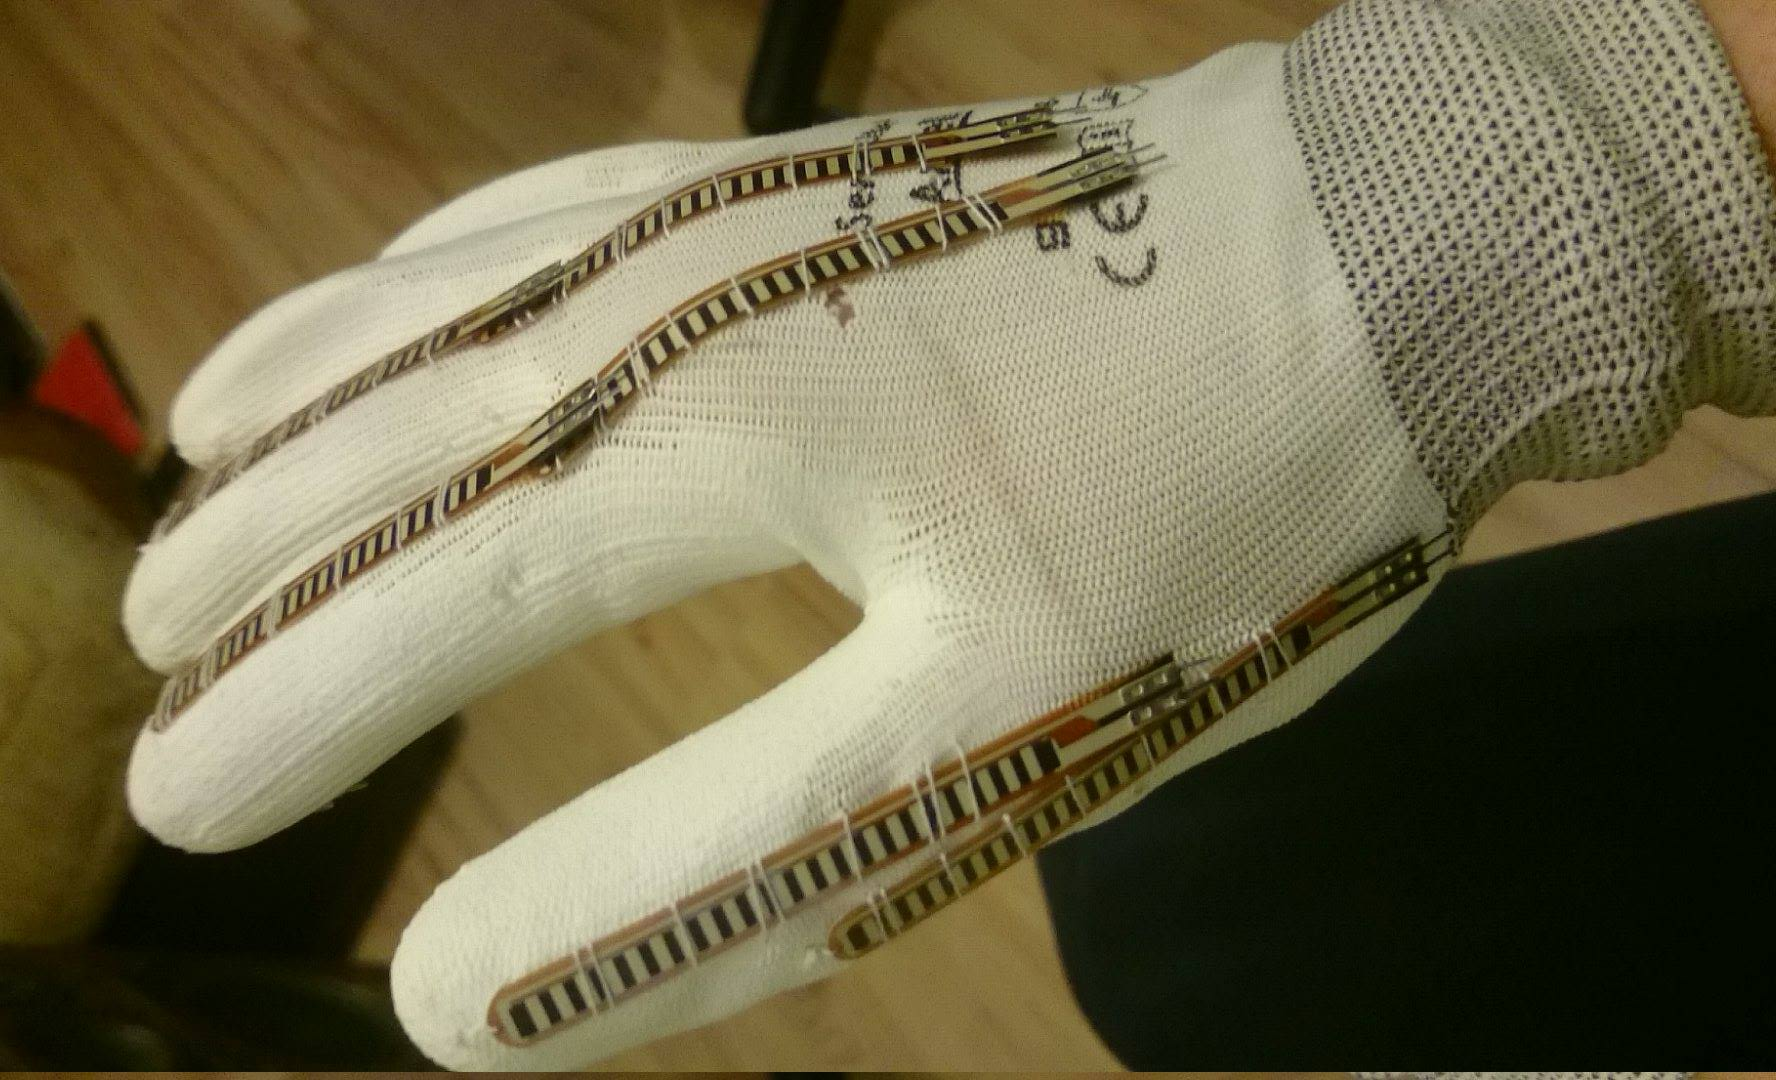
\includegraphics[width=0.65\textwidth]{images/rekawica2.jpg}
\caption{Zdjęcie rękawicy w fazie montażu (aktualny rozkład czujników jest zmieniony)}
\label{fig:rekawica2}
\end{figure}


\subsubsection{Płytka sterująca}
Do sterowania pomiarami i połączeniem z komputerem wykorzystano płytkę STM32DiscoveryF3. Na płytce znajduje się mikrokotroler STM32F303VCT6, którego piny wyprowadzone są na podwójne listwy goldpin. Dokumentację oraz schemat połączeń płytki można znaleźć na stronie producenta. Wygląd płytki oraz rozmieszczenie elementów ukazano na rysunku [rys.\ref{fig:discovery}].\\
Płytka została umieszczona na rękawicy na przyszytych żeńskich listwach goldpin, co umożliwia używanie jej jako moduł i odłączenie od urządzenia.
\begin{figure}[!htb]
\centering
\begin{subfigure}{.5\textwidth}
	\centering
	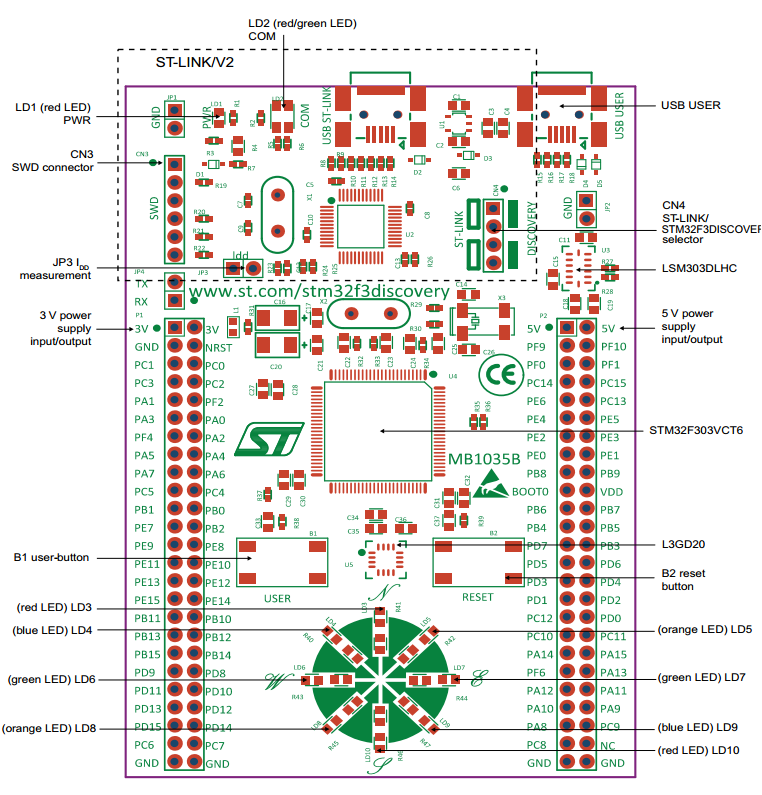
\includegraphics[height=.35\textheight]{images/stm32f3layout.png}
	\caption{Rozmieszczenie elementów}
	\label{fig:gotowa}
\end{subfigure}%
\begin{subfigure}{.5\textwidth}
	\centering
	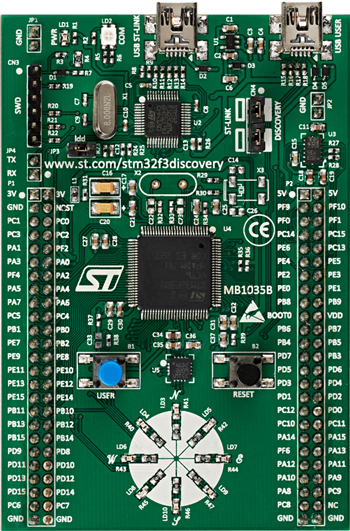
\includegraphics[height=.35\textheight]{images/32f3discovery.jpg}
	\caption{Wygląd płytki}
	\label{fig:gotowa2}
\end{subfigure}
\caption{Główna płytka sterująca}
\label{fig:gotowa_rekawica}
\end{figure}

\subsubsection{Czujniki}
Opis czujników został przedstawiony w rozdziale \textit{Opis czujników}. Aby umożliwić pomiar stworzono dzielniki napięciowe dla czujników, których schemat został przedstawiony na rysunku [rys.\ref{fig:dzielnik}].
\begin{figure}[!htb]
\centering
\includegraphics[width=.8\textwidth]{./images/Dzielniki.png}
\caption{Schematy dzielników napięciowych do pomiarów \label{fig:dzielnik}}
\end{figure}

\subsubsection{Komunikacja}

\subsubsection{Przewody}
Do realizacji połączeń elektrycznych wykorzystano cienkie przewody wielożyłowe. Ideowy schemat połączeń został przedstawiony na rysunku [rys. \ref{fig:kabelki}].
\begin{figure}[!htb]
\centering
\includegraphics[width=.8\textwidth]{./images/SchematIdeowy.png}
\caption{Ideowy schemat połączeń na płytce \label{fig:kabelki}}
\end{figure}


\subsection{Software}
\subsubsection{Struktury danych}
Dane z czujników są przechowywane w następujących strukturach:
\begin{figure}[!htb]
\begin{lstlisting}[frame=single]
#define FINGER_JOINT_COUNT 3
#define FINGER_COUNT 5

#define FLEX_SENSOR_COUNT 10
#define TENSION_SENSOR_COUNT 5
#define ACCELEROMETER_AXIS_COUNT 3
#define SENSOR_COUNT (FLEX_SENSOR_COUNT+TENSION_SENSOR_COUNT+ACCELEROMETER_AXIS_COUNT)


typedef struct s_measurements
{
	uint16_t FlexSensor[FLEX_SENSOR_COUNT];
	uint16_t TensionSensor[TENSION_SENSOR_COUNT];
	int16_t Accelerometer[ACCELEROMETER_AXIS_COUNT];
} s_measurements;

typedef struct s_AggregatedMeasurements
{
	float FlexSensor[FLEX_SENSOR_COUNT];
	uint8_t TensionSensor[TENSION_SENSOR_COUNT];
	float Accelerometer[ACCELEROMETER_AXIS_COUNT];
} s_AggregatedMeasurements;

typedef struct s_JointAngles
{
	float Joint[FINGER_JOINT_COUNT];
} s_JointAngles;
\end{lstlisting}

\end{figure}

\subsection{Wizualizacja}
\subsubsection{Interfejs graficzny}
Aplikacja pozwala na wizualizację modelu ręki na podstawie odczytów z czujników. Powstała we frameworku Qt. Aktualny interfejs graficzny wyświetla uproszczony model dłoni [rys. \ref{fig:wds}].

\begin{figure}[htb!]
\centering
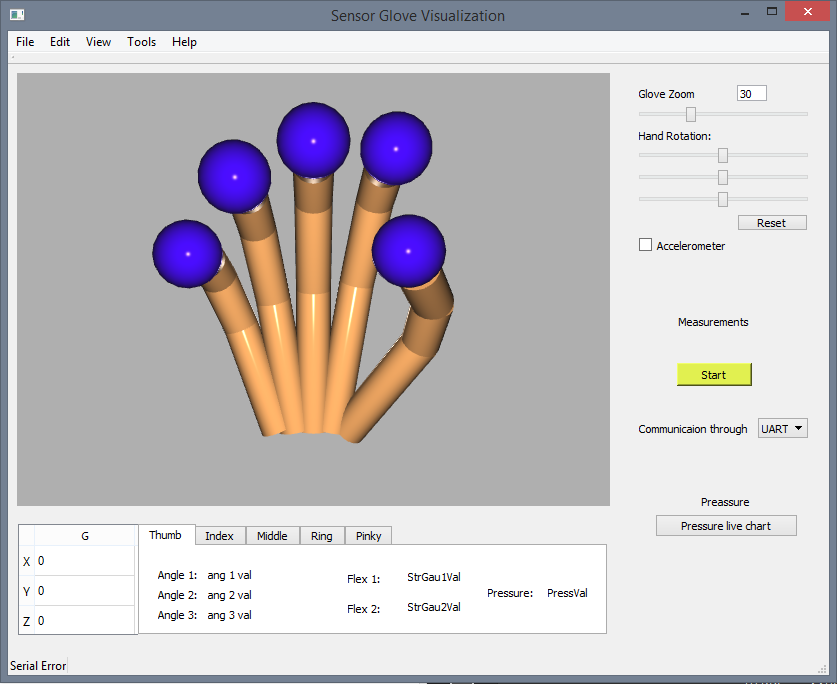
\includegraphics[width=0.8\textwidth]{images/aktualnyinterfejsgraficzny.png}
\caption{Aktualny interfejs graficzny}
\label{fig:wds}
\end{figure}

\subsubsection{Funkcjonalności aplikacji}
Zostanie stworzona aplikacja okienkowa do wizualizacji napisana w języku C++ z użyciem biblioteki Qt.\\
\begin{itemize}
\item Wizualizacja poruszania modelem dłoni na podstawie odczytów z czujników i akcelerometru.
\item Wybór opcji połączenia z rękawicą sensoryczną (Bluetooth, USB, UART)
\item Uruchomienie i zatrzymanie pomiarów, wykonanie pojedynczego pomiaru.
\item Skalowanie modelu dłoni poprzez wpisanie rozmiarów oraz suwak.
\item Zmiana położenia i orientacji kamery z poziomu interfejsu graficznego.
\item Zmiana rotacji modelu dłoni (RPY) poprzez suwaki interfejsu graficznego.
\item Wyświetlanie liczbowo wyników pomiarów i możliwość zapisania ich do pliku.
\item Wyświetlenie dynamicznego wykresu odczytu nacisku wybranego palca w czasie.
\end{itemize}

\subsection{Pomiary} %Trochę poleciałaś z tym czasem rzeczywistym :D
Projekt umożliwia podglądanie następujących parametrów w programie STMStudio:\\\\
\textbf{Dane z czujników nacisku:}
\begin{itemize}
\item Wyrażone w woltach
\item Zobrazowane za pomocą przestrzeni kolorów HSV
\end{itemize}
\textbf{Dane z czujników ugięcia:}
\begin{itemize}
\item Wyrażone w woltach
\item Interpolowane liniowo na kąty w przegubach
\end{itemize}
\textbf{Dane z akcelerometru:}
\begin{itemize}
\item Wyrażone w $m/s^2$
\end{itemize}
Powyższe wartości są filtrowane na bieżąco przez filtr dolnoprzepustowy ze zmiennym parametrem $\beta$ (zależnie od metody wysyłania).
\begin{equation} \label{eq:1}
y[n] - \beta y[n-1] = (1-\beta)x[n]
\end{equation}
Nastawy przegubów są interpolowane funkcją liniową na podstawie pomiarów w skrajnych przypadkach maksymalnego i minimalnego zgięcia. Pomiary obarczone są dużym błędem ze względu na niestabilność konstrukcji (przesuwanie się czujników) oraz trudność w dobraniu metody pomiarowej. Pomiary przedstawiono poniżej.
\begin{itemize}
\item \textbf{Kciuk}\\
Minimalne wartości odczytów czujników: 2500,1850\\
Maksymalne wartości odczytów czujników: 2130,2500\\
Minimalne zmierzone wartości kątów w przegubach: 0.0,0.0,0.0\\
Maksymalne zmierzone wartości kątów w przegubach: 90.0,45.0,70.0\\

\item \textbf{Palec wskazujący}\\
Minimalne wartości odczytów czujników: 1920,1800\\
Maksymalne wartości odczytów czujników: 2760,3200\\
Minimalne zmierzone wartości kątów w przegubach: 0.0,0.0,0.0\\
Maksymalne zmierzone wartości kątów w przegubach: 85.0,130.0,55.0\\

\item \textbf{Palec środkowy}\\
Minimalne wartości odczytów czujników: 1920,1650\\
Maksymalne wartości odczytów czujników: 2650,2880\\
Minimalne zmierzone wartości kątów w przegubach: 0.0,0.0,0.0\\
Maksymalne zmierzone wartości kątów w przegubach: 90.0,120.0,70.0\\

\item \textbf{Palec serdeczny}\\
Minimalne wartości odczytów czujników: 1750,1560\\
Maksymalne wartości odczytów czujników: 2300,2300\\
Minimalne zmierzone wartości kątów w przegubach: 0.0,0.0,0.0\\
Maksymalne zmierzone wartości kątów w przegubach: 80.0,100.0,85.0\\

\item \textbf{Palec mały}\\
Minimalne wartości odczytów czujników: 1520,1440\\
Maksymalne wartości odczytów czujników: 2580,2930\\
Minimalne zmierzone wartości kątów w przegubach: 0.0,0.0,0.0\\
Maksymalne zmierzone wartości kątów w przegubach: 90.0,90.0,90.0\\
\end{itemize}

\begin{figure}[htb!]
\centering
\begin{subfigure}{.5\textwidth}
	\centering
	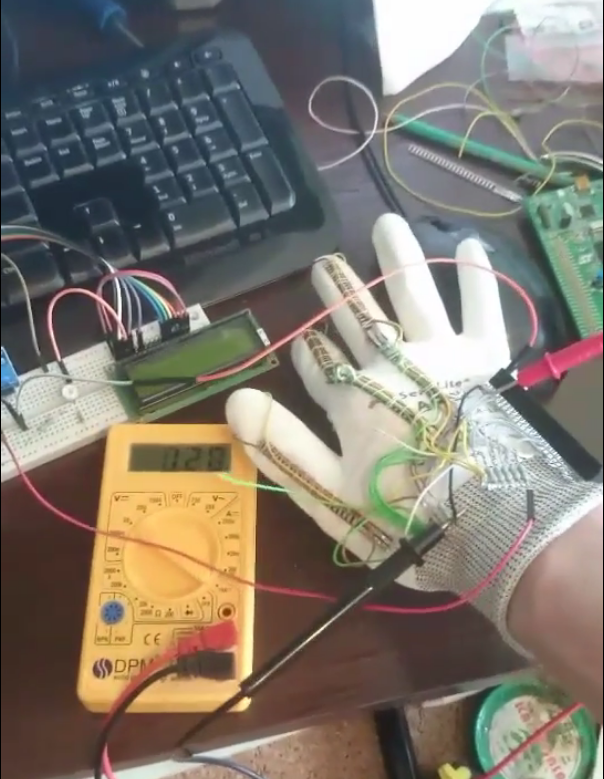
\includegraphics[width=.9\textwidth]{images/nacisk.png}
	\caption{Testowanie czujników nacisku}
	\label{fig:nacisk}
\end{subfigure}%
\begin{subfigure}{.5\textwidth}
	\centering
	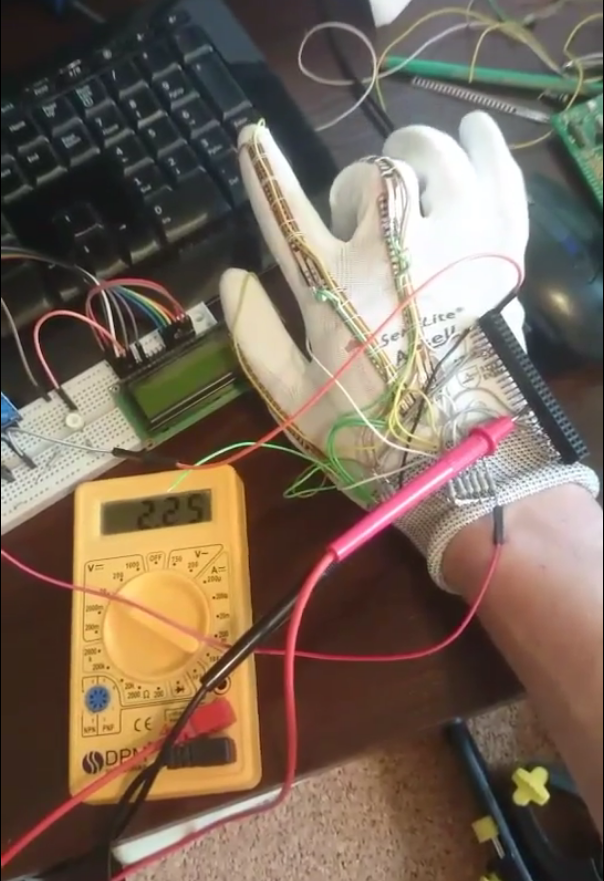
\includegraphics[width=.9\textwidth]{images/ugiecie.png}
	\caption{Testowanie czujników ugięcia}
	\label{fig:ugiecie}
\end{subfigure}
\caption{Testy}
\label{fig:testy}
\end{figure}

\newpage
\section{Badania z wykorzystaniem rękawicy}
Rękawica sensoryczna pozwala na zbieranie pomiarów i próbę jak najdokładniejszego wykrycia konkretnych gestów ludzkiej dłoni na podstawie odczytów z czujników. Takie badania mogą być wykorzystywane m.in. przy rozwoju protez biomedycznych. Takie gesty mogą posłużyć sterowaniu robotem lub systemem automatyki (np. budynkowej). Przyporządkowanie gestu do wykonywanej czynności daje możliwość kontroli systemu.\\
Wykrywanie gestów sprowadza się do ustawienia odpowiednich progów na niektórych czujnikach ugięcia i nacisku, po których przekroczeniu sygnalizuje się wykrycie gestu.\\

\subsection{Dane pomiarowe}
Zbadano poprawność pozyskiwania i wysyłania danych pomiarowych za pomocą terminala (Realterm) oraz programu STMStudio. Wyniki przedstawiono na rysunkach (\ref{fig:term}, \ref{fig:stmstudio}).\\
\begin{figure}
\centering
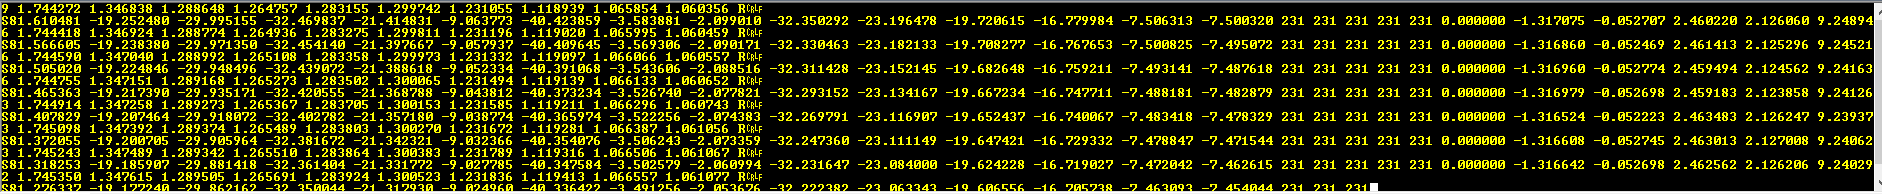
\includegraphics[width=\textwidth]{./images/terminal.png}
\caption{Wysyłane dane wyświetlone na terminalu \label{fig:term}}
\end{figure}
\begin{figure}
\centering
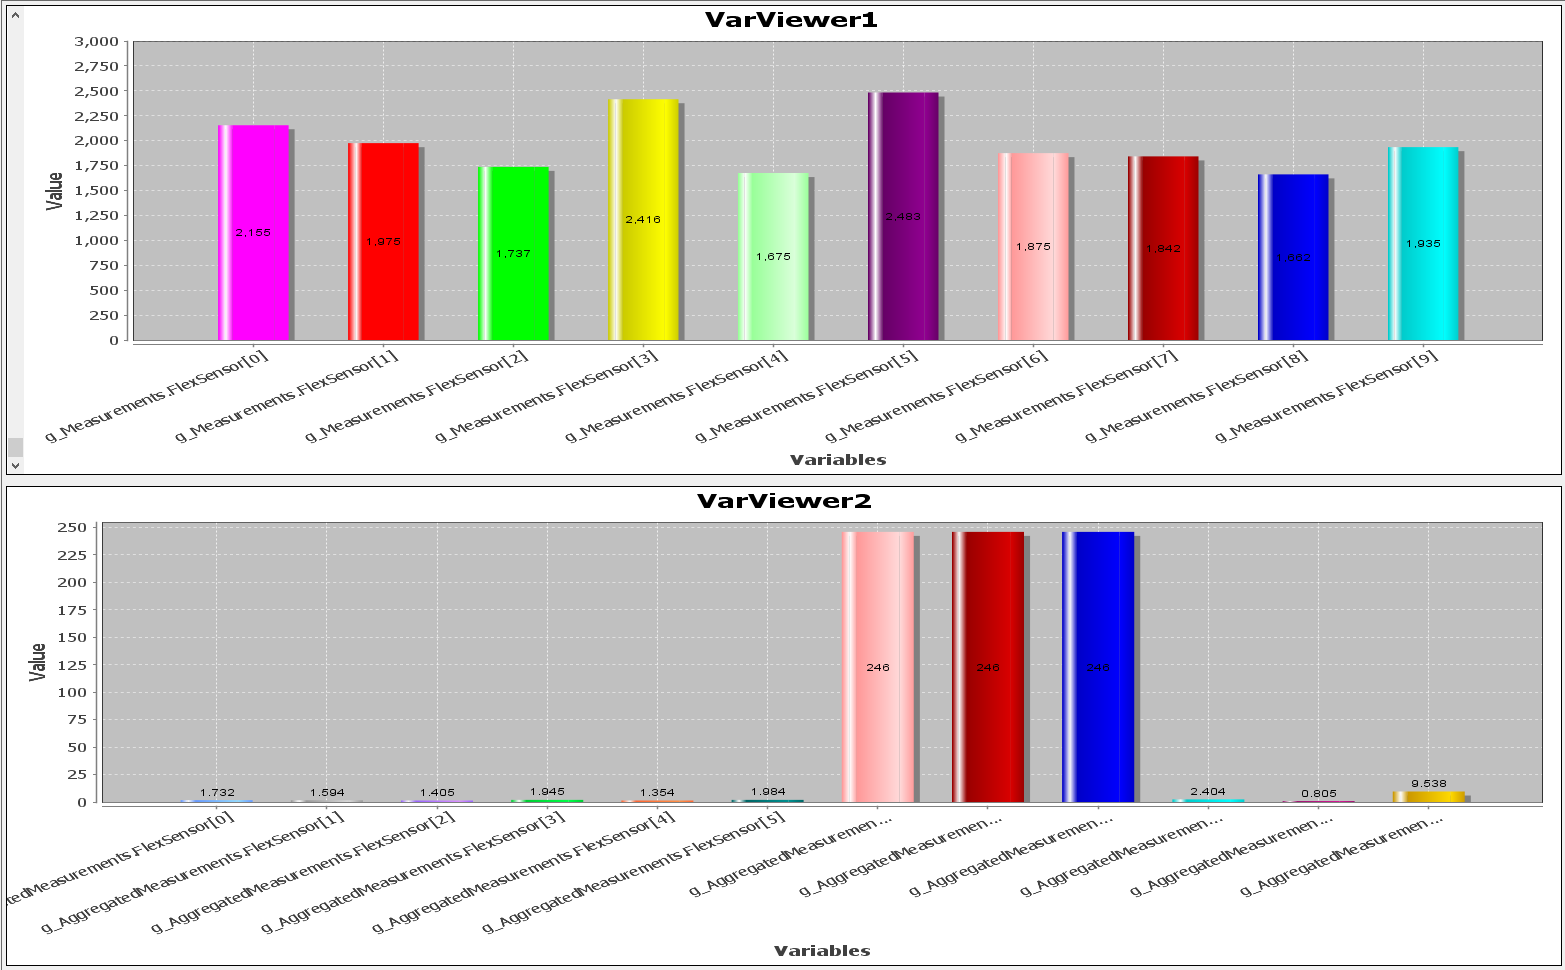
\includegraphics[width=\textwidth]{./images/stmstudio.png}
\caption{Pobierane dane wyświetlone w STMStudio\label{fig:stmstudio}}
\end{figure}

\subsection{Przykładowe gesty}
Badane gesty zostały przedstawione na rysunkach (\ref{fig:Fist}, \ref{fig:Palm}, \ref{fig:OK}, \ref{fig:Peace}, \ref{fig:Point}).\\
\begin{figure}[!htb]
\centering
    \begin{subfigure}{.5\textwidth}
    \centering
      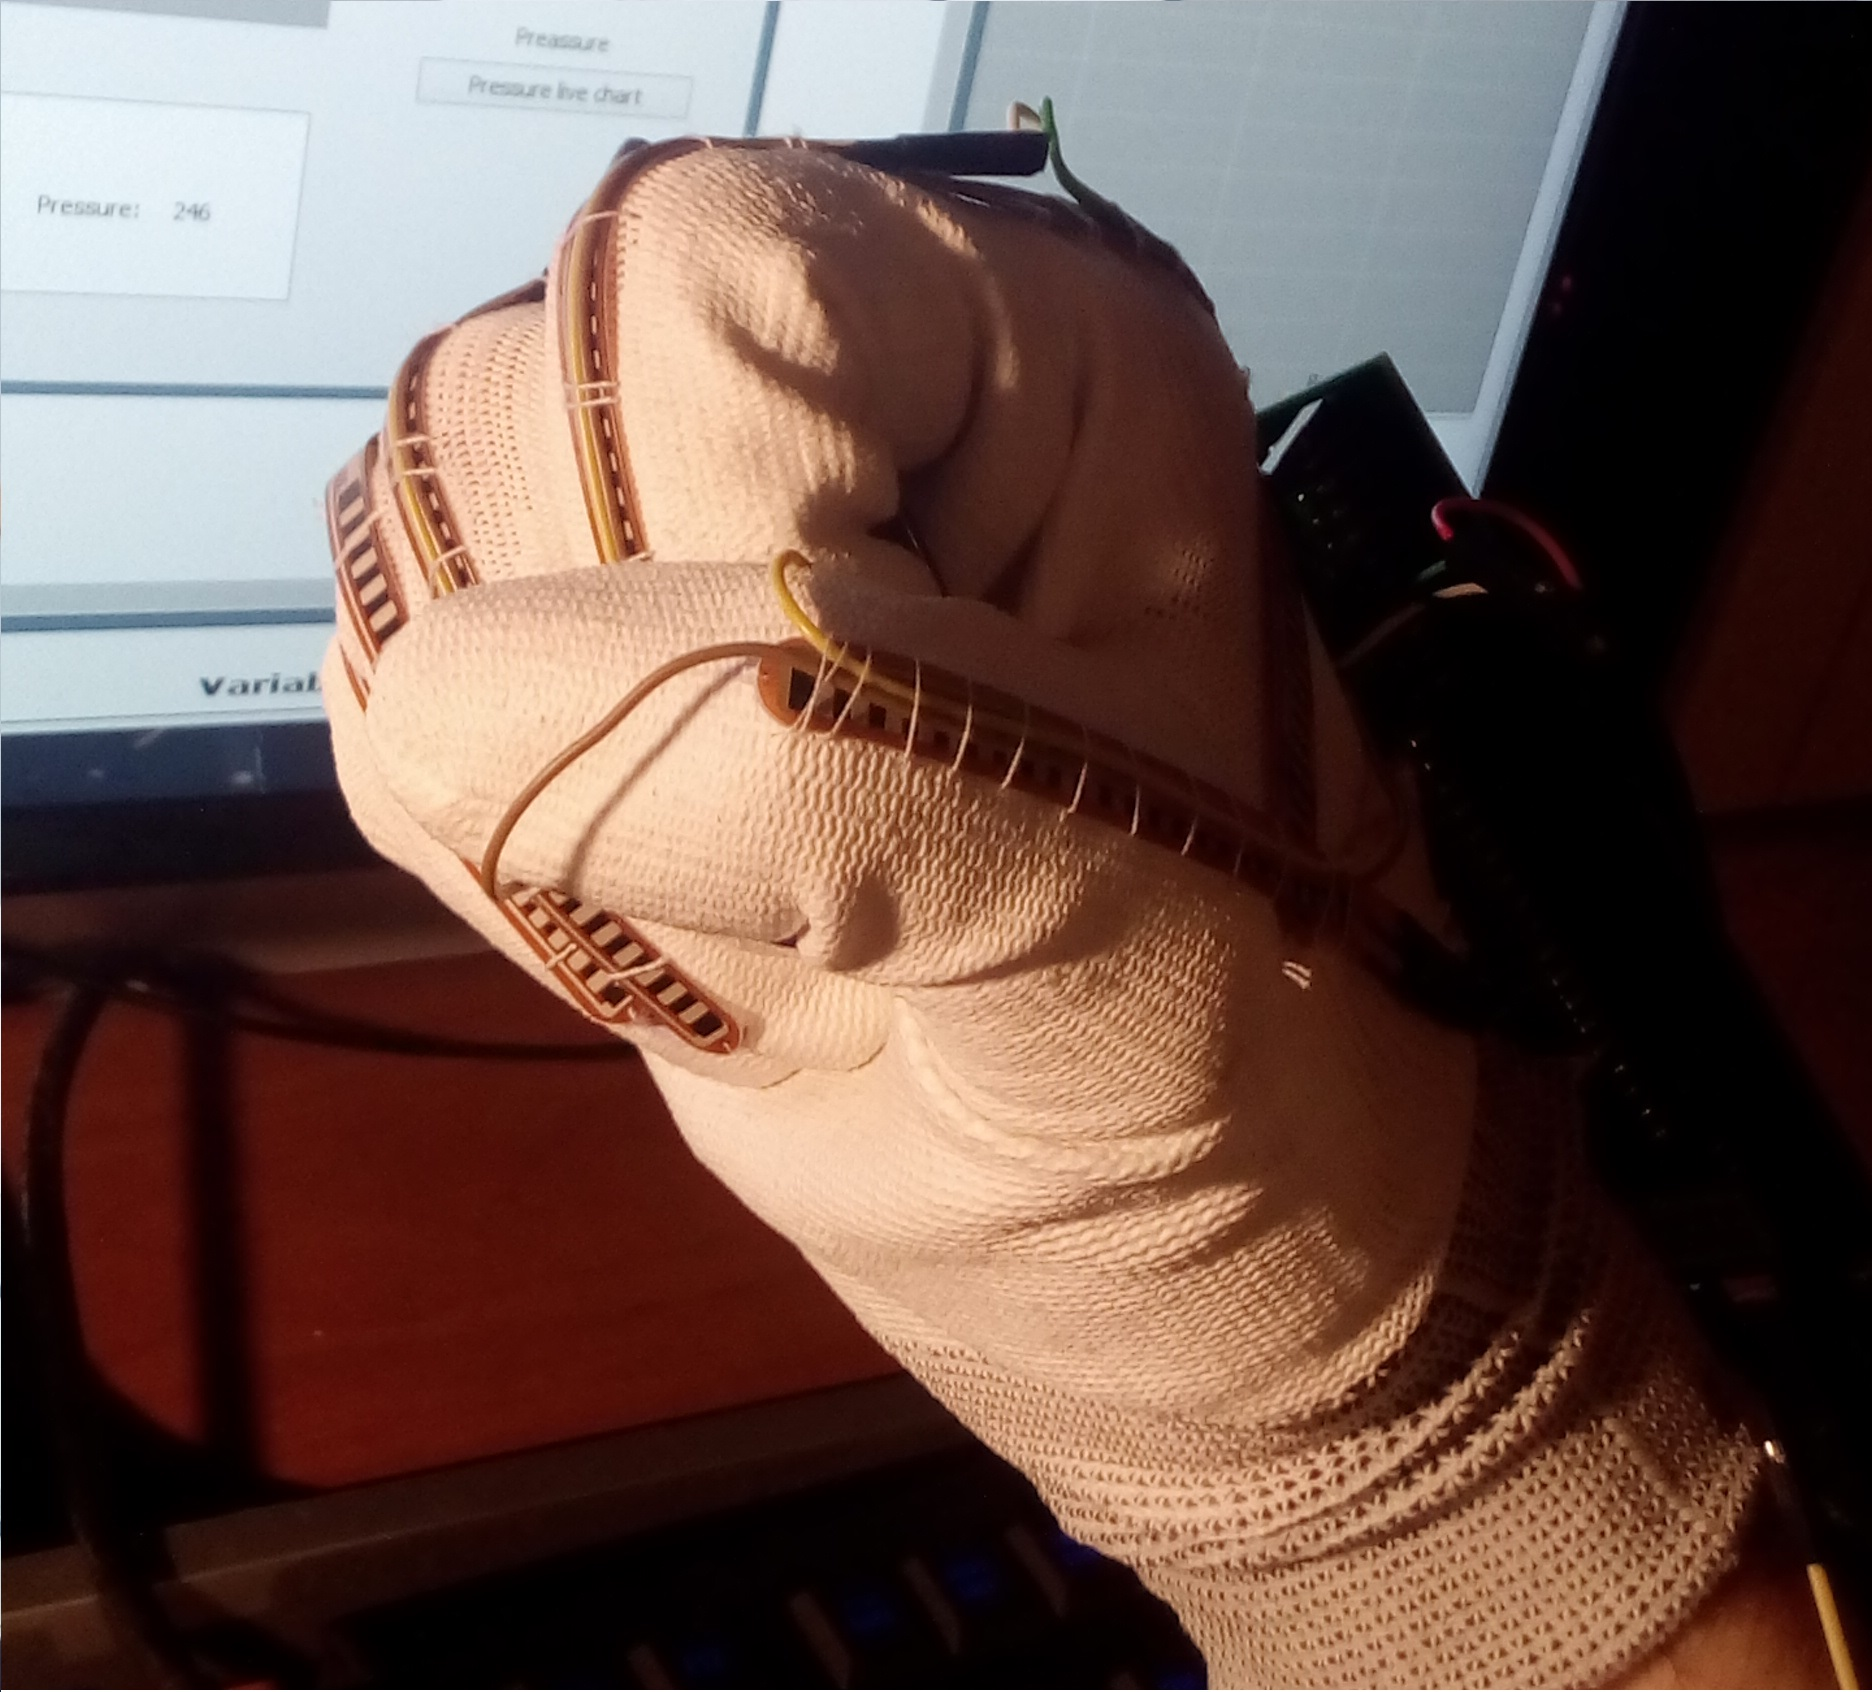
\includegraphics[width=0.9\textwidth]{./images/Fist.jpg}
     \end{subfigure}%
    \begin{subfigure}{.5\textwidth}
    \centering
      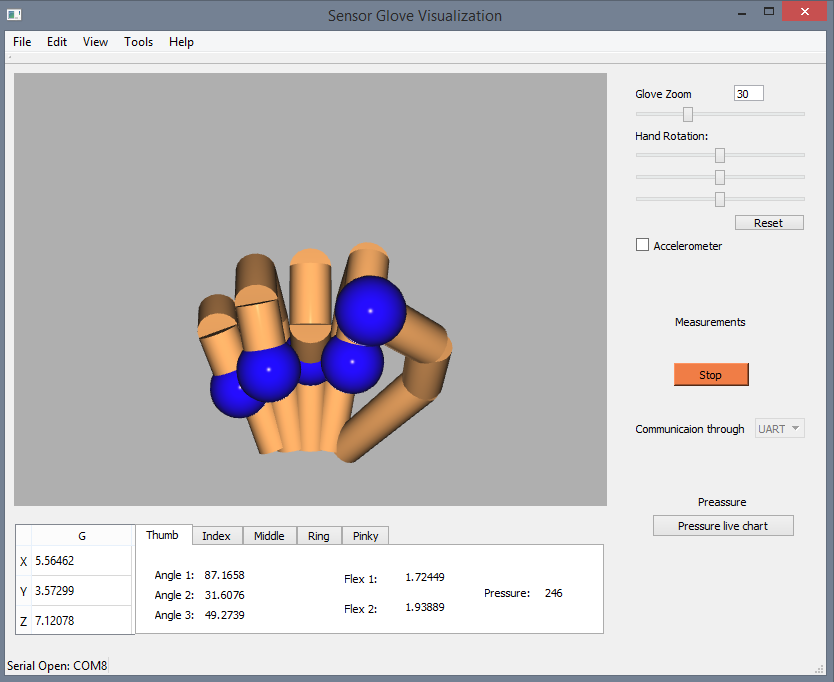
\includegraphics[width=0.9\textwidth]{./images/FistQt.png}
     \end{subfigure}
    \caption{Gest -- zaciśnięta pięść \label{fig:Fist}}
\flushleft Metoda identyfikacji: Kąty we wszystkich przegubach przekraczają określoną wartość.
\end{figure}

\begin{figure}[!htb]
\centering
    \begin{subfigure}{.5\textwidth}
      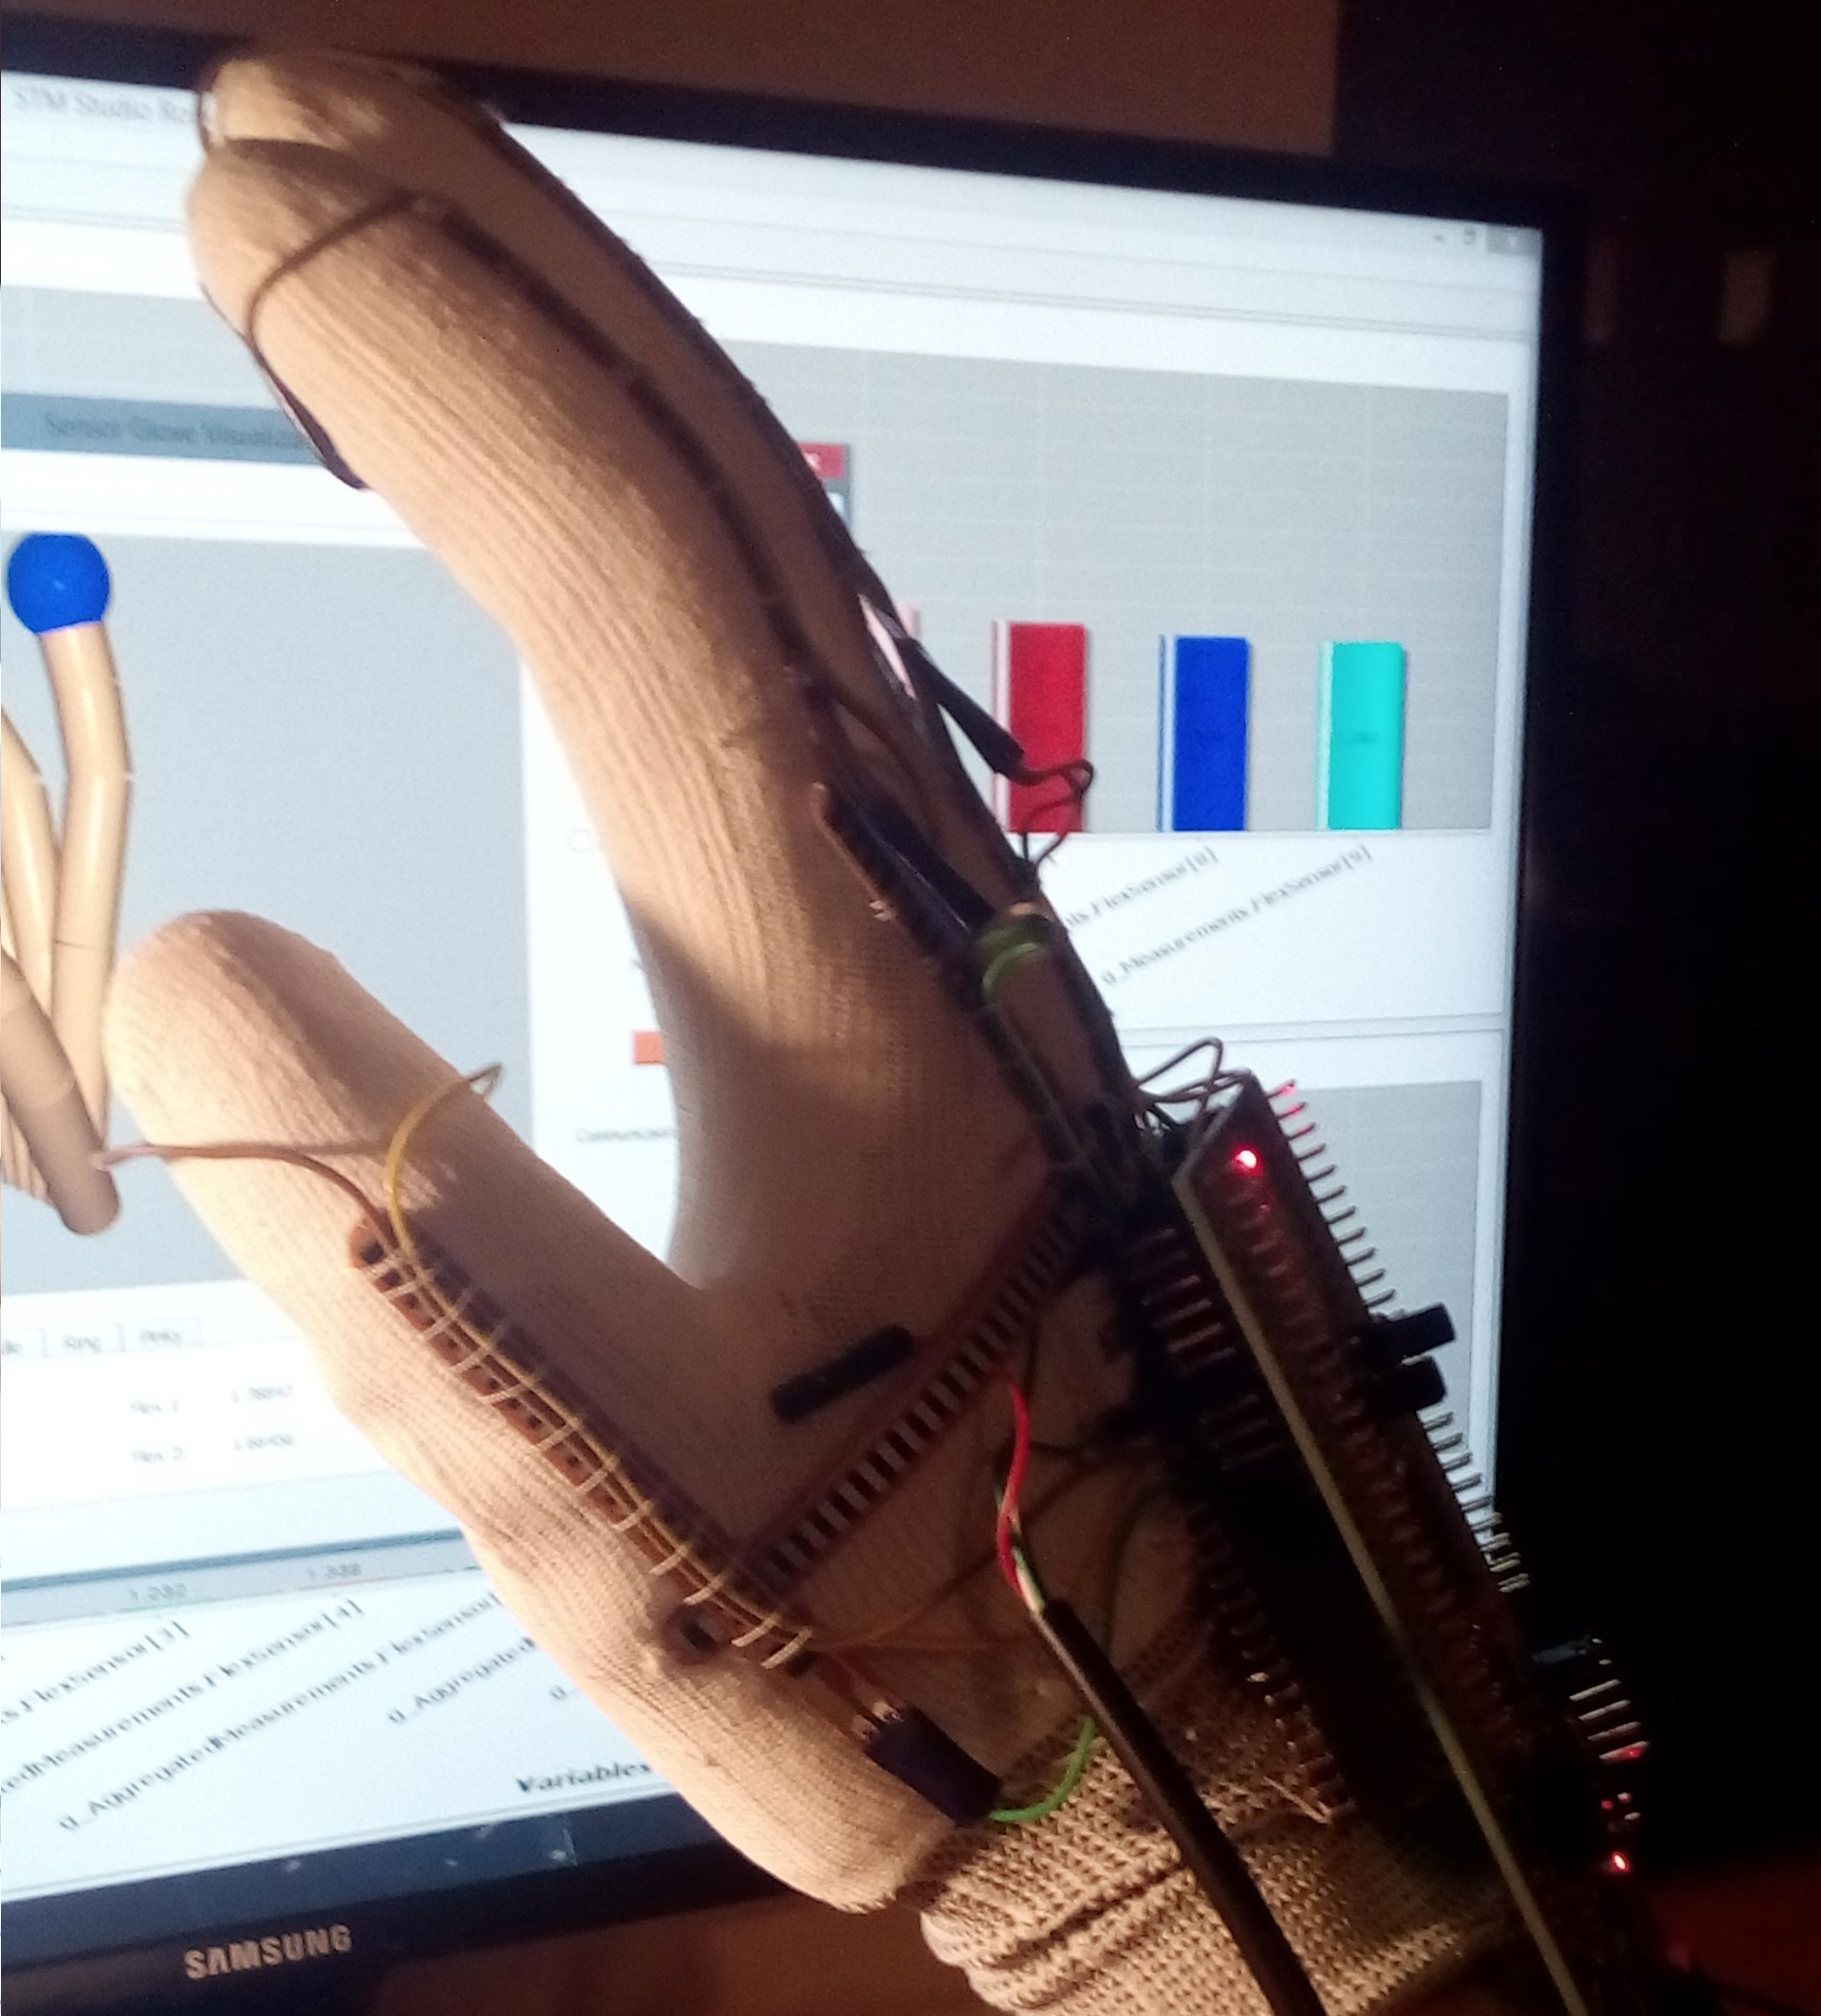
\includegraphics[width=0.9\textwidth]{./images/Palm.jpg}
     \end{subfigure}%
    \begin{subfigure}{.5\textwidth}
      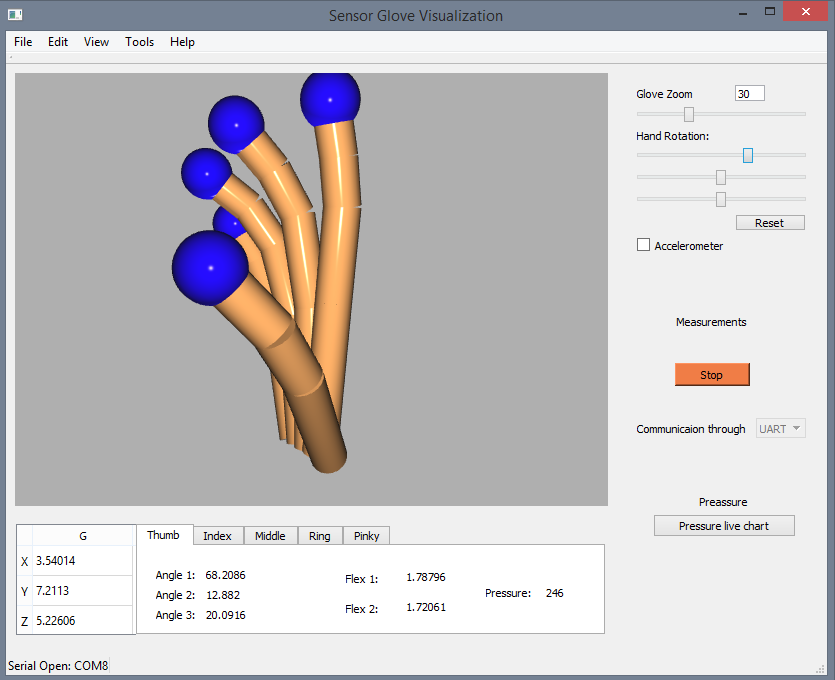
\includegraphics[width=0.9\textwidth]{./images/PalmQt.png}
     \end{subfigure}
    \caption{Gest -- otwarta dłoń \label{fig:Palm}}
\flushleft Metoda identyfikacji: Kąty we wszystkich przegubach nie przekraczają określonej wartości.
\end{figure}

\begin{figure}[!htb]
\centering
    \begin{subfigure}{.5\textwidth}
      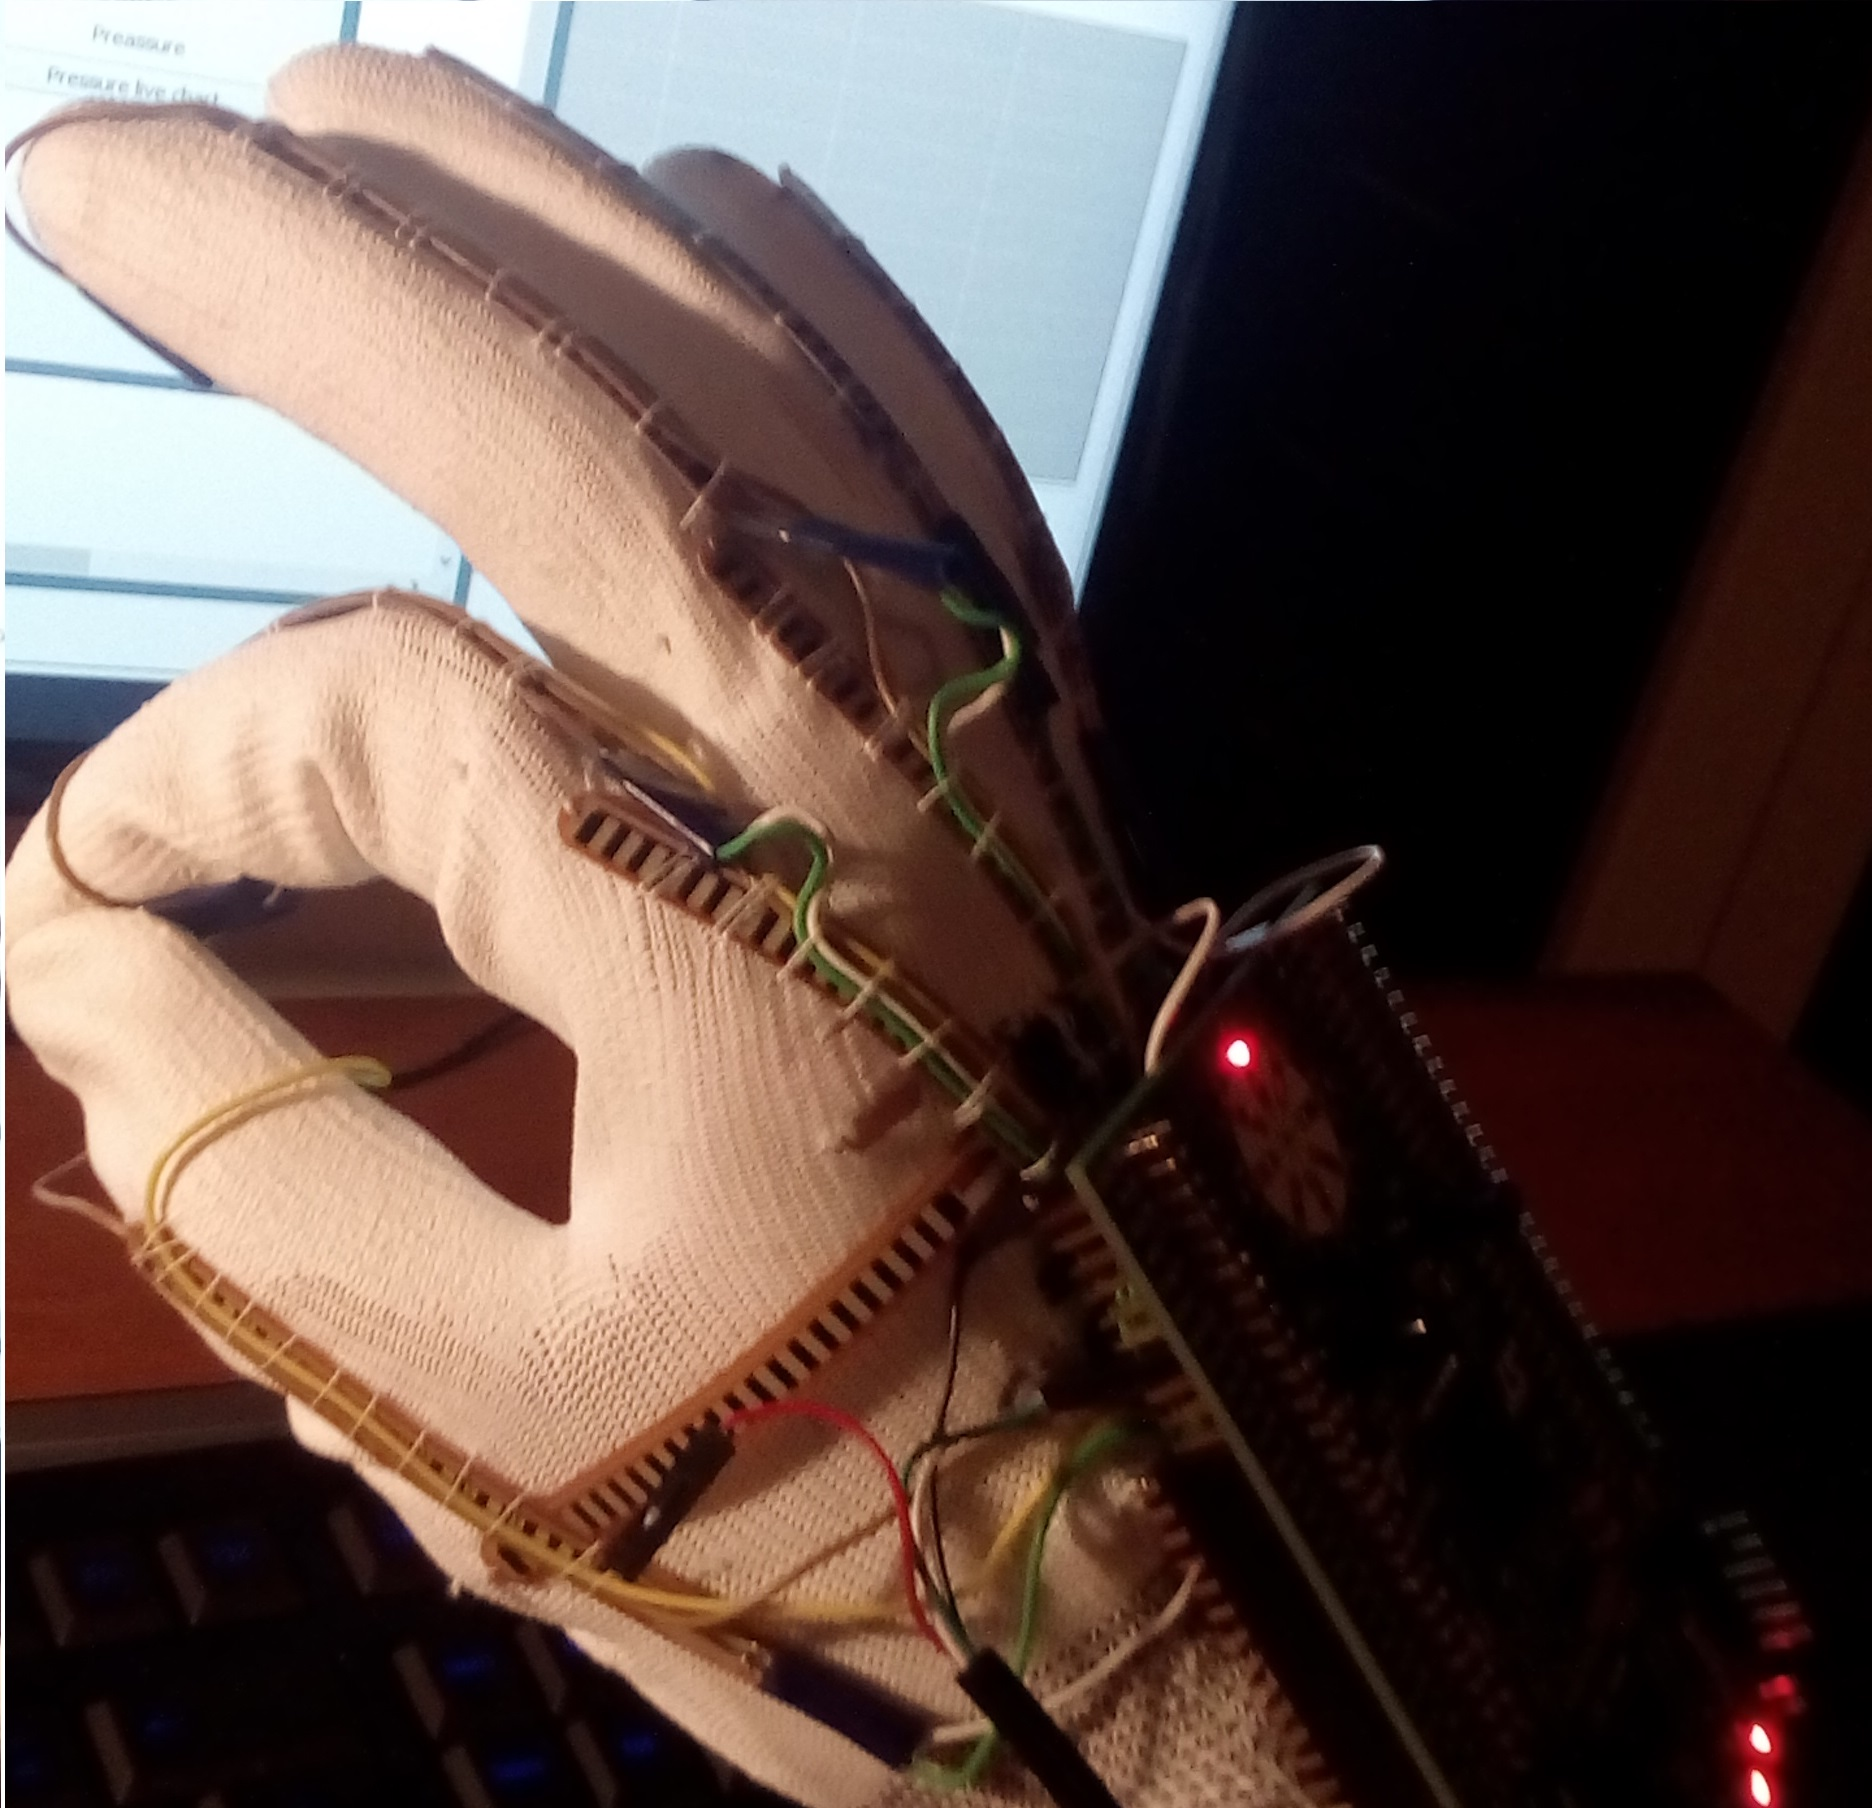
\includegraphics[width=0.9\textwidth]{./images/OK.jpg}
     \end{subfigure}%
    \begin{subfigure}{.5\textwidth}
      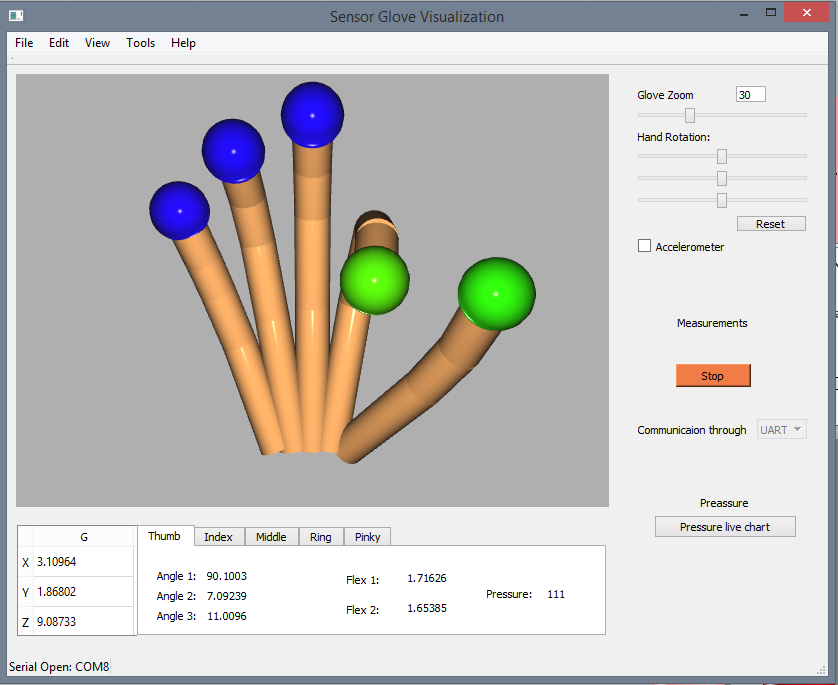
\includegraphics[width=0.9\textwidth]{./images/OKQt.png}
     \end{subfigure}
    \caption{Gest -- OK \label{fig:OK}}
\flushleft Metoda identyfikacji: Nacisk na palcach przekracza określona wartość.
\end{figure}

\begin{figure}[!htb]
\centering
    \begin{subfigure}{.5\textwidth}
      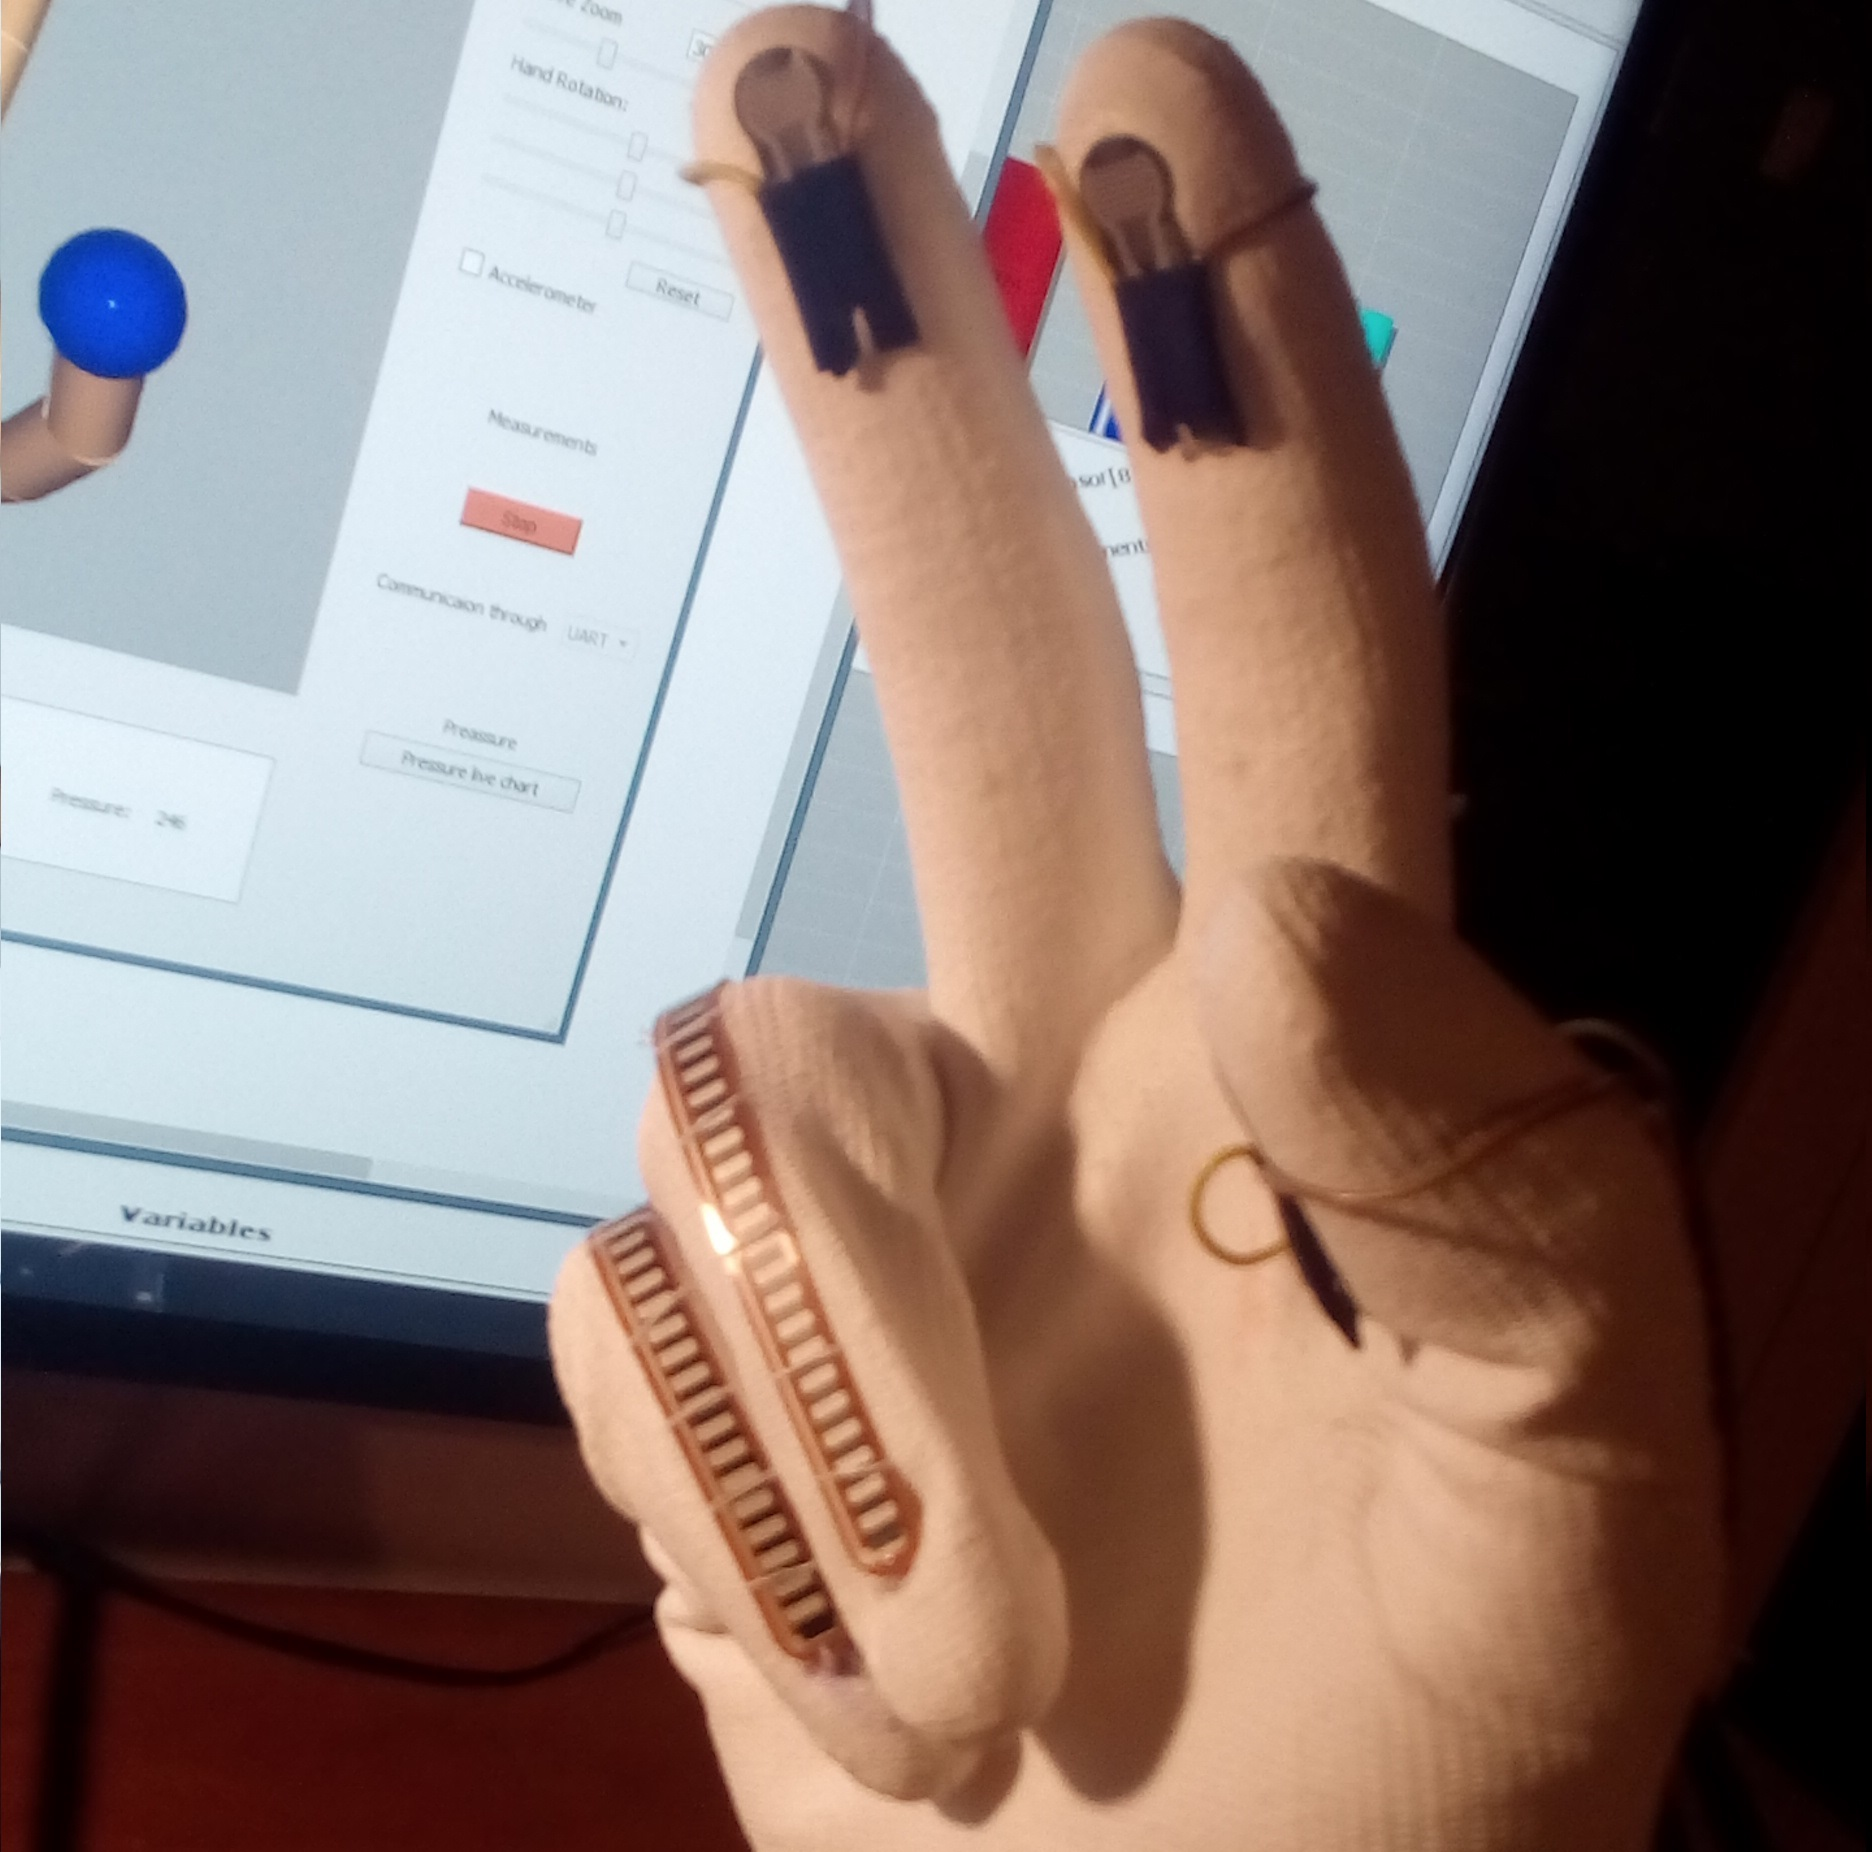
\includegraphics[width=0.9\textwidth]{./images/Peace.jpg}
     \end{subfigure}%
    \begin{subfigure}{.5\textwidth}
      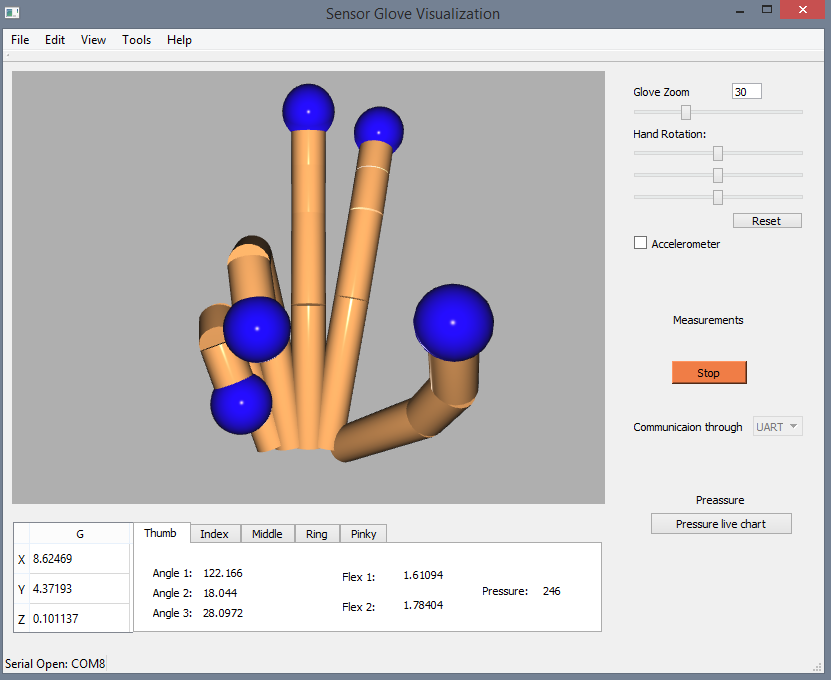
\includegraphics[width=0.9\textwidth]{./images/PeaceQt.png}
     \end{subfigure}
    \caption{Gest -- pacyfka\label{fig:Peace}}
\flushleft Metoda identyfikacji: Kąty w przegubach kciuka oraz palców wskazującego i środkowego nie przekraczają określonej wartości. Kąty w przegubach palców serdecznego i małego przekraczają określoną wartość.
\end{figure}

\begin{figure}[!htb]
\centering
    \begin{subfigure}{.5\textwidth}
      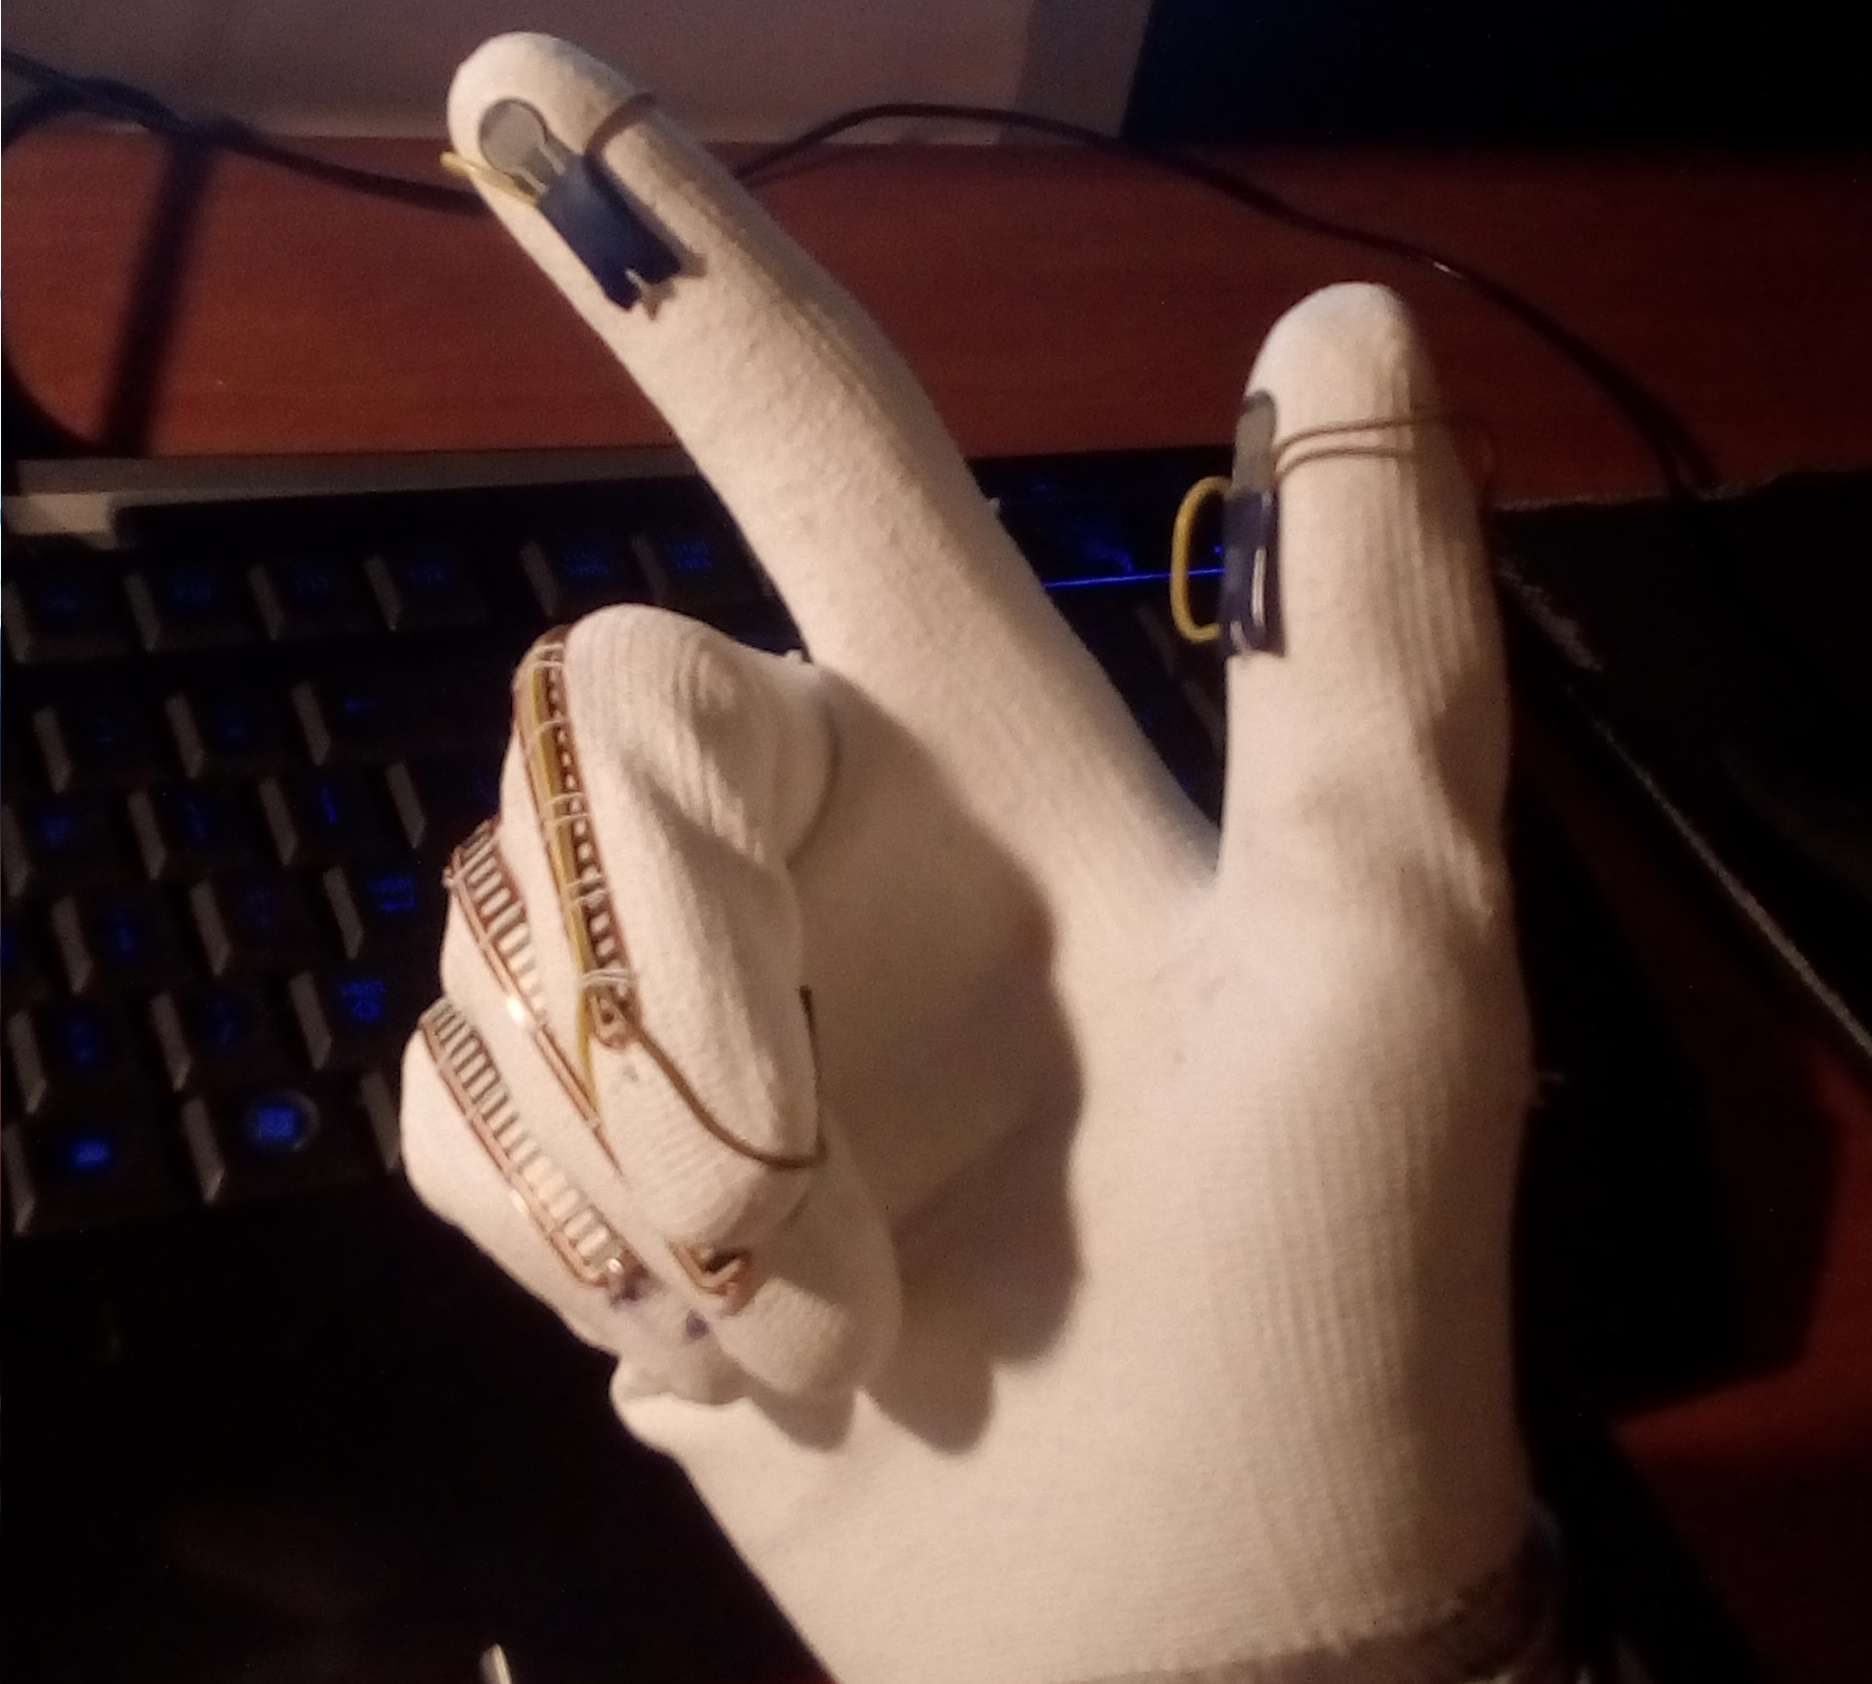
\includegraphics[width=0.9\textwidth]{./images/Point.jpg}
     \end{subfigure}%
    \begin{subfigure}{.5\textwidth}
      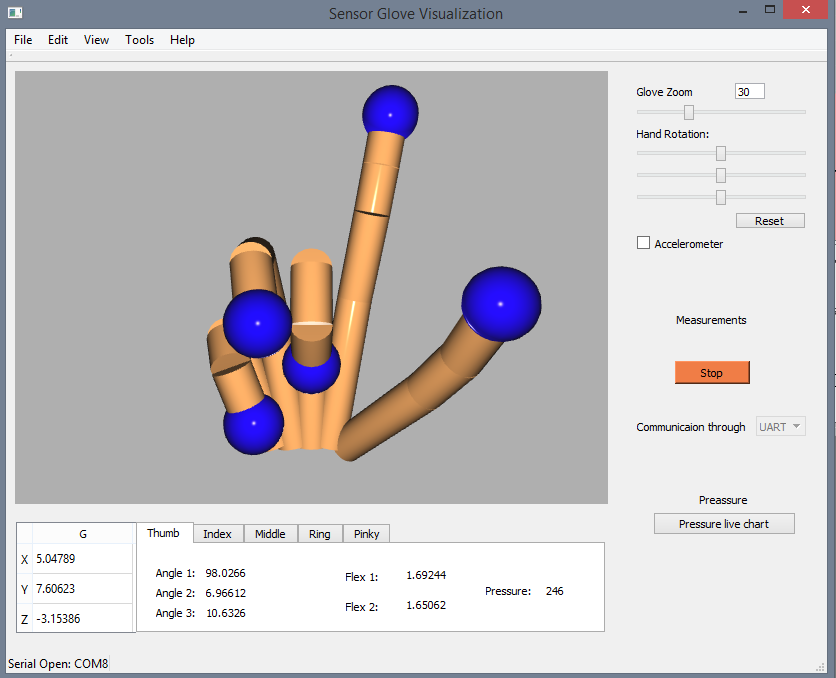
\includegraphics[width=0.9\textwidth]{./images/PointQt.png}
     \end{subfigure}
    \caption{Gest -- wskazywanie palcem \label{fig:Point}}
\flushleft Metoda identyfikacji: Kąty w przegubach kciuka oraz palców środkowego, serdecznego i małego przekraczają określoną wartość. Kąty w przegubach palców wskazującego i kciuka nie przekraczają określonej wartości.
\end{figure}

\newpage
\section{Podsumowanie}
\subsection{Problemy podczas konstrukcji}
\begin{itemize}
\item \textit{Mała powierzchnia czujników nacisku} -- przy niektórych chwytach człowiek wykorzystuje różne części palców, np. powierzchnię boczną, a czujniki umieszczone są tylko na opuszkach
\item \textit{Problem z umieszczeniem czujnika rotacji kciuka} -- jest to złożony ruch, trudno wychwycić go jednym wąskim czujnikiem
\item \textit{Różnice w dłoniach konstruktorów} -- rękawica musi pasować do konkretnej dłoni, żeby czujniki były na odpowiednich miejscach i poprawnie zbierały pomiary
\item \textit{Mała dokładność czujników, przesuwanie się ich na rękawicy}
\item \textit{Niedoskonałość pomiarów kątów zgięcia palców} -- przy danej konstrukcji i typie czujników nie jest możliwe uzyskanie tak wysokiej dokładności, jak zakładano
\item \textit{Trudności w uzyskaniu poprawnego działania aproksymacji kątów z akcelerometru}
\item \textit{Kłopoty z interpolacją / aproksymacją} -- jest to trudne do uzyskania w C
\item \textit{Komplikacje przy zamówieniu elementów elektronicznych na katedrę} -- brak kontaktu z laborantem sprawił, że przez pewien czas nie można było uzyskać informacji, czy zamówienie zostało złożone, co poskutkowało opóźnieniem projektu
\end{itemize}
\subsection{Zmiany w założeniach projektowych}
\begin{itemize}
\item \textit{Zamontowanie na opuszkach LEDów wizualizujących odczyty z czujników nacisku} -- zabrakło miejsca, bo czujniki trzeba było przesunąć w stosunku do wstępnego schematu, a poza tym każda dioda wymagałaby 4 kabli, co utrudniałoby ruchy dłoni
\item \textit{Bezprzewodowe przesyłanie danych do komputera za pomocą modułu Bluetooth} -- zrezygnowano, bo okazało się za wolne (BaudRate 9600 nie wystarcza)
\end{itemize}
\subsection{Pomysły na rozwinięcie projektu}
\begin{itemize}
\item RPY z wielu akcelerometrów
\item Dokładniejsze pomiary i metoda interpolacji
\item Wykrywanie większej ilości gestów
\item Sterowanie robotem za pomocą gestów
\item Dodatkowe czujniki nacisku
\end{itemize}

\end{document}
